% This is a template for the assignment reports
% TARI29 Artificial Intelligence, 7.5 credits, Winter 2024
% Original version by:  Vladimir Tarasov, 2024
% Revised by:           Alexandros Tzanetos, 2024 

% Use a modern class instead of an old article class
\documentclass{scrartcl}

\KOMAoptions{
    parskip=half,  % full, off
    fontsize=12pt, % base font size (10pt default)
    % headings=big,% small/normal/big headings (normal is default), 
    % paper=a5,    % paper format (a4 default) 
    pagesize=auto  % Use paper format for PDF too
}

% ---------------------- Report details --------------------- %
%\newcommand{\docauthor}{Name1, Name2, Name3}
\newcommand{\courseyear}{2025}
\newcommand{\coursename}{TARI29 Artificial Intelligence}
\newcommand{\coursecredits}{7.5 credits}
\newcommand{\fullcoursename}{\coursename, \coursecredits}
\newcommand{\termname}{Winter \courseyear}
\newcommand{\groupnumber}{6}
\newcommand{\reportname}{Group \groupnumber\ Assignment Report}
\newcommand{\assignmentname}{Evolutionary Computation Assignment}
% ------------------ End of report details ------------------ %



% ---------- Setting up properties of the PDF file ---------- %
\usepackage{hyperref}
\hypersetup{
    colorlinks=true,
    allcolors=blue,
    pdftitle={\reportname},
    pdfauthor={Name1, Name2, Name3},
    pdfsubject={\coursename, \termname}
	% pdfpagemode=FullScreen,
	% pdfpagemode= UseOutlines % the default if present
}
% ------------ End of properties of the PDF file ------------ %



% ----------- Setting up the headers and footers ------------ %
\usepackage{scrlayer-scrpage}
\pagestyle{scrheadings}
\KOMAoptions{% 
    headsepline,% line below the header
    plainheadsepline,% also on scrplain
}
\clearscrheadfoot % Erase all current configurations
% inner part of the header [titel_page]{other_pages}
\ihead[\coursename, \courseyear]{\coursename, \courseyear}
% outer part of the header [titel_page]{other_pages}
\ohead{\assignmentname}
% center part of the footer [titel_page]{other_pages}
\cfoot[\textup{Page \pagemark\ of \ztotpages}]{\textup{Page \pagemark\ of \ztotpages}}
% ------------- End of the headers and footers -------------- %



% ---------------- Setting up the title page ---------------- %
\title{\reportname}
\subtitle{An Evolutionary Algorithm for solving Sudokus}
%\author{\docauthor}
\author{Ben Bekir Ertugrul \and Eduard Iorga \and Haoran Liu \and Moritz Schlitter
}
\date{\today}
% ------------------ End of the title page ------------------ %

\usepackage[english]{babel}

% --------------- Packages and custom commands -------------- %
% Specify the input encoding of the source file as UTF8 
\usepackage[utf8]{inputenc}
% The T1 font encoding is an 8-bit encoding and fully supports words containing accented characters
\usepackage[T1]{fontenc}
% Load Latin modern fonts in outline format
\usepackage{lmodern}
% Load better typewriter font
\usepackage{inconsolata}
% For better hyphenation patterns
\usepackage[english]{babel}
% For improved micro-typography
\usepackage{microtype}
% Switch off extra space after a sentence
\frenchspacing
% To be able to iclude pictures
\usepackage{graphicx}
\usepackage{adjustbox}
\usepackage{subcaption}
\usepackage{zref-totpages} % To get the total number of pages
\usepackage{mathtools,amsmath} % for advanced math formulas
 % To highlight source code
\usepackage{minted}
% Default options for all minted environments
\setminted{
           style=default, % for minted envronment
           autogobble, % automatically remove all common leading whitespace
           xleftmargin=10pt, % indentation to add (on the left) before the listing
           numbersep=6pt, % gap between numbers and start of line
           linenos, % enables line numbers
           mathescape % enables the usual math mode inside comments
}
\setmintedinline[c]{style=default} % for minted inlines
% Flexible handling of verbatim text
\usepackage{fancyvrb}
% For well-spaced lines and guidelines in tables
\usepackage{booktabs}
% To typeset algorithms or pseudocode in LaTeX 
\usepackage{algorithm}
\usepackage{algpseudocode}
% For plots and graphs
\usepackage{pgfplots}
\pgfplotsset{width=10cm,compat=1.9}
% For visualizing sudoku puzzles
\usepackage{sudoku}

% To generate placeholder text - can be deleted when you have written real text
\usepackage{lipsum}
% ----------- End of packages and custom commands ----------- %

\begin{document}

\maketitle

% % It can be commented out if you do not want the table of contents
% \tableofcontents 

\section{Introduction}
\label{sec:intro}

Traditionally, a Sudoku is a logic based number placement puzzle. The objective of the puzzle is to fill a most commonly 9x9 sized grid with digits so that each column, row and 3x3 subgrid contain all of the digits from 1 to 9.\cite{}

Solving such a puzzle programmatically falls into the category of search and optimization problems. These types of problems can be approached in different ways. One possible approach is depicted by evolutionary algorithms or in this case more specifically, genetic algorithms (GA)\cite{WikiSudoku}.

Inspired by the process of natural selection, GAs use biologically inspired operators such as selection, crossover and mutation to generate solutions to optimization and search problems\cite{WikiGA}.

This paper studies the efficiency of solving Sudoku puzzles with GA approaches. The objective is to compare the performance of different implementations of GAs. These approaches will additionally be compared to the naive search algorithm depth-first search (DFS). The puzzles explored will be of different difficulties for regular 9x9 grids and bigger 16x16 and 25x25 grids. This way the paper analyzes whether GAs are a viable option for efficiently solving Sudoku boards compared to naive search algorithms as the complexity of the puzzle increases.

This document is organized in the following way. Chapter one describes the objective of this study. Chapter two describes the problem of solving Sudoku puzzles and the motivation of using evolutionary algorithm approaches to solve this type of problem. Chapter three details the algorithm used in this study. The following chapter lays out the setup of the experiments run in this study. Lastly, chapter five presents and analyses the results of this paper.
\section{Sudoku Puzzle Problem}
\label{sec:problem_description}
\subsection{Problem Description}
{Sudoku is a Japanese logical game that is played on a $9 \times 9$ grid, that are further divided into $3 \times 3$ subgrids. The objective of the game is to fill the grid with digits from 1 to 9, ensuring that each row, column, and subgrid contains each digit exactly once\cite{Mantere2007}. The puzzle starts with some cells already filled in, and the player must use logic and respect the base rule of the game in order to finish the puzzle.}
{\newline}
{\newline Sudoku puzzles can vary in difficulty based on how many numbers they start with, the arrangement of these numbers and even the varying size of the sudoku, since they can go beyond the standard $9 \times 9$ grid, similar to the $25 \times 25$ grid we used to test our algorithm with. Thus we can think of the sudoku problem as a graph coloring problem if it were to be expressed in a mathematical context. The $9 \times 9$ grid can be seen as graph that has 81 vertices, namely one vertex for each cell. Each vertex can be labeled with an ordered pair (x,y), where x and y are integers between 1 and 9 \cite{WikiMathematics}. Two distinct vertices (x1,y1) and (x2,y2) are connected by an edge if and only if they are in the same row, column or subgrid:}
\begin {itemize}
    \item $x1 = x2$, which translates as same row
    \item $y1 = y2$, which translates as same column
    \item $\lfloor (x1-1)/3 \rfloor = \lfloor (x2-1)/3 \rfloor$ and $\lfloor (y1-1)/3 \rfloor = \lfloor (y2-1)/3 \rfloor$ which translates as same subgrid
\end {itemize}
{As previously mentioned, the puzzle is completed when all the vertices have an integer between 1 and 9 assigned to them, in such a way that vertices that are joined by an edge don't have the same number assigned to them. }
\subsection{Evolutionary Approach}
{While Sudoku has a deterministic solution, evolutionary algorithms can be used in order to compare their performance with more traditional approaches such as the depth first search algorithm. As it is mentioned in\cite{Moraglio}, they managed to implement an evolutionary algorith that could solve very efficently easy Sudoku puzzles. The downside of their algorithm, was that it wasn't as efficient when it came down to solving medium or hard puzzles.   }
{\color{red}
\begin{itemize}
    \item The mathematical formulation considered in your study. Some problems have a clear mathematical model (e.g., Travelling Salesman Problem), while others do not (e.g., $n$-Queens). Based on the problem you chose, search the literature and find a proper way to present the problem.
    \item One paragraph that briefly presents at least 3 published academic works where any evolutionary approach is used to solve the problem. It would be wise to cite here works that influenced your algorithm. This practice saves you time from looking for additional academic resources. You can find more information about reading and searching in the literature in \cite{zobel2014reading}.
    \item The motivation behind the evolutionary approach you decided to develop. A good practice would be to align the motivation with some literature gap found in the academic works you presented above. However, this is not mandatory. You can motivate your selection on the characteristics of the algorithm making it proper for the problem.
\end{itemize}
}

\textcolor{red}{\textbf{Note:} Change the section's title to match the name of the problem you chose for your assignment.}

---

- This section presents the problem this paper solves with the use of evolutionary algorithm approach. 

- Math in solving Sudokus? Maybe rather introducing quickly a sudoku, how to solve it and describing the steep increase of difficulty with increasing sizes of sudoku puzzles

- Cite 3 published papers. Cite where our idea is from\cite{Mantere2007}. Another Paper\cite{Amil2019}.

- Motivation behind evolutionary approach.



\section{Genetic Algorithm}
\label{sec:algorithm}

\textcolor{red}{The third section should present the evolutionary approach you developed. You can divide this section into subsection. In any case, you should mention the following details:}

\textcolor{red}{\textbf{Evolutionary approach.} Clearly describe the algorithm you developed. You should clearly explain the evolutionary operators you used and what modifications you did to match the problem. It is extremely important to present also a pseudocode of your algorithm. An example is given in \ref{alg:pseudocode_example}, below. For more insight into presentation of algorithms, you can advise \cite{zobel2014algorithms}.}

{
\color{red}To typeset pseudocode in \LaTeX\ you can use one of the following options:
\begin{itemize}
    \item Choose ONE of the (\texttt{algpseudocode} OR \texttt{algcompatible} OR \texttt{algorithmic}) packages to typeset algorithm bodies, and the algorithm package for captioning the algorithm.
    \item The \texttt{algorithm2e} package.
\end{itemize}
You can find more information here: \url{https://www.overleaf.com/learn/latex/Algorithms}
}

\begin{algorithm}
\caption{Example of an algorithm's pseudocode}\label{alg:pseudocode_example}
\begin{algorithmic}
\Require $n \geq 0$
\Ensure $y = x^n$
\State $y \gets 1$
\State $X \gets x$
\State $N \gets n$
\While{$N \neq 0$}
\If{$N$ is even}
    \State $X \gets X \times X$
    \State $N \gets \frac{N}{2}$  \Comment{This is a comment}
\ElsIf{$N$ is odd}
    \State $y \gets y \times X$
    \State $N \gets N - 1$
\EndIf
\EndWhile
\end{algorithmic}
\end{algorithm}

\textcolor{red}{\textbf{Solution representation.} Clearly describe the solution representation you used. You can use figures to improve the comprehensibility of this part.}

\textcolor{red}{\textbf{Fitness function.} It is also very important to mention the fitness function you used. In many cases, the objective function of the problem is not the same as the fitness function used in an evolutionary algorithm. An example, following the principles of \cite{zobel2014mathematics}, is given below.}

\begin{equation}
    F = \sum_{i=1}^d x_i^2 
\end{equation}
where $x_i$ is the $i$-th gene (i.e., decision variable) in the solution and $d$ corresponds to the number of decision variables in the problem.

\textcolor{red}{\textbf{Note:} Change the section's title to match the name of the algorithm you developed for your assignment.}

\subsection{Implementations}
This section presents and compares different implementations of an evolutionary algorithm designed to solve Sudoku puzzles. Each implementation varies in its approach to selection, crossover, mutation strategies, and fitness evaluation.

The following sections document these processes and use the Sudoku board shown in \ref{fig:initial-sudoku} as a reference for visualizing the selection and mutation step.

\begin{figure}[H]
\centering
\resizebox{0.5\textwidth}{!}{
  \begin{minipage}{\textwidth}
    \begin{sudoku}
    | |2| | | | | |3|1|.
    |7| | | | |3| | | |.
    | | | |1|4| |2|9| |.
    | |5|2|7|6|4| |1|8|.
    | |6|3| |1|2|7|5|9|.
    | |7|8| | | |4| | |.
    |2| | |3|7| | | |5|.
    | |1| | | | |9| | |.
    |5|4| | |8|1| | | |.
    \end{sudoku}
  \end{minipage}%
}
\caption{Initial Sudoku puzzle}
\label{fig:initial-sudoku}
\end{figure}

\subsubsection{Baseline}
Depth-first search (DFS) is used as a deterministic baseline. The solver iteratively scans the board for the first empty cell, attempts candidate values 1\dots n, and backtracks to try alternative values if no candidate leads to a solution. This approach is ensures a solution (given that the puzzle is solvable) and is simple to implement, which makes it a reliable reference for correctness and for measuring runtimes.
Algorithm \ref{alg:dfs} shows the implementation of the DFS algorithm in pseudo-code.

\begin{algorithm}[H]
\caption{Depth-first search algorithm}\label{alg:dfs}
\begin{algorithmic}
\Require matrix
\Ensure \textbf{true} if solved, \textbf{false} otherwise
\State $n \gets$ length(matrix)
\For{$i \leftarrow 1$ \textbf{to} $n$}
  \For{$j \leftarrow 1$ \textbf{to} $n$}
    \If{matrix[$i,j$] = 0}
      \For{$num \leftarrow 1$ \textbf{to} $n$}
        \If{is\_valid\_move(matrix, $i$, $j$, $num$)}
          \State matrix[$i,j$] $\gets$ $num$
          \If{\Call{DFS}{matrix}} \State \Return \textbf{true} \EndIf
          \State matrix[$i,j$] $\gets$ 0
        \EndIf
      \EndFor
      \State \Return \textbf{false}
    \EndIf
  \EndFor
\EndFor
\State \Return \textbf{true}
\end{algorithmic}
\end{algorithm}

\pagebreak % TODO: make sure this is properly formatted, but if we dont pagebreak here, then the next paragraph might appear above the table, which is not good.
\subsubsection{Implementation 1}\label{sec:impl-1}

Algorithm \ref{alg:impl-1} gives an overview of how the algorithm works. A detailed description of how the fitness function, crossover, and mutation work, will be given afterwards.

\begin{algorithm}[H]
\caption{Genetic Algorithm 1}\label{alg:impl-1}
\begin{algorithmic}
\Require $initial\_sudoku$, $population\_size$, $mutation\_rate$, $max\_generations$
\Ensure Best individual found
\State $population \gets$ PopulateRandomly($initial\_sudoku$, $population\_size$)
\State $generation \gets 0$
\While{$generation < max\_generations$}
  \State $population \gets$ SortByFitness($population$) \Comment{descending order}
  \If{Fitness(first($population$)) = $max\_fitness$}
    \State \Return first($population$)
  \EndIf
  \State $next\_generation \gets \emptyset$
  \For{$i \gets 1 \ \textbf{to} \ population\_size \times 0.8$}
    \State $parent_1, parent_2 \gets$ Sample(top 20\% of $population$)
    \State $child \gets$ Crossover($parent_1$, $parent_2$)
    \State $child \gets$ Mutate($child$, $mutation\_rate$, $initial\_sudoku$)
    \State $next\_generation \gets next\_generation \cup \{child\}$
  \EndFor
  \For{$i \gets 1 \ \textbf{to} \ population\_size \times 0.2$}
    \State $parent_1, parent_2 \gets$ Sample($population$)
    \State $child \gets$ Crossover($parent_1$, $parent_2$)
    \State $child \gets$ Mutate($child$, $mutation\_rate$, $initial\_sudoku$)
    \State $next\_generation \gets next\_generation \cup \{child\}$
  \EndFor
  \State $population \gets next\_generation$
  \State $generation \gets generation + 1$
\EndWhile
\State $population \gets$ SortByFitness($population$) \Comment{descending order}
\State \Return first($population$)
\end{algorithmic}
\end{algorithm}


\paragraph{Fitness function}\label{par:ff-impl1} The fitness function evaluates a Sudoku board by summing the number of unique digits in each row, column, and 3$\times$3 block, with a maximum score of 243 for a valid solution.
{
  \color{red} TODO
}
\begin{equation}
    F = \sum_{i=1}^d x_i^2 
\end{equation}

\paragraph{Crossover} A new individual is creating by crossing over two parents. The crossover process simply iterates over all the tiles that were not given in the initial puzzle and takes the value for that tile from either parent to copy it to the child.

\begin{figure}[H]
  \centering
  {\setlength{\tabcolsep}{-9pt}
  \renewcommand{\arraystretch}{1.5}
   \begin{tabular}{c c c c c}
    % first board
    \begin{adjustbox}{width=0.38\textwidth,valign=c}
      \begin{minipage}{\linewidth}
        \begin{sudoku}
        |6|2|9|5|7|6|7|3|1|.
        |7|8|5|6|9|3|1|2|7|.
        |1|3|4|1|4|7|2|9|5|.
        |4|5|2|7|6|4|4|1|8|.
        |9|6|3|8|1|2|7|5|9|.
        |9|7|8|2|9|5|4|6|2|.
        |2|2|6|3|7|7|9|4|5|.
        |4|1|6|2|2|3|9|7|9|.
        |5|4|1|2|8|1|3|4|8|.
        \end{sudoku}
      \end{minipage}
    \end{adjustbox}
    & % plus sign
    {\begin{adjustbox}{valign=c}\Large$+$\end{adjustbox}}
    &
    % second board
    \begin{adjustbox}{width=0.38\textwidth,valign=c}
      \begin{minipage}{\linewidth}
        \begin{sudoku}
        |8|2|6|7|7|5|7|3|1|.
        |7|1|3|9|8|3|8|2|4|.
        |1|5|5|1|4|7|2|9|3|.
        |9|5|2|7|6|4|1|1|8|.
        |4|6|3|9|1|2|7|5|9|.
        |3|7|8|5|9|1|4|6|3|.
        |2|8|7|3|7|1|7|4|5|.
        |3|1|6|4|2|3|9|7|2|.
        |5|4|4|2|8|1|3|4|3|.
        \end{sudoku}
      \end{minipage}
    \end{adjustbox}
    & % equals sign
    {\begin{adjustbox}{valign=c}\Large$=$\end{adjustbox}}
    &
    % third board
    \begin{adjustbox}{width=0.38\textwidth,valign=c}
      \begin{minipage}{\linewidth}
        \begin{sudoku}
        |8|2|9|7|7|6|7|3|1|.
        |7|1|5|6|8|3|1|2|4|.
        |1|3|5|1|4|7|2|9|5|.
        |9|5|2|7|6|4|1|1|8|.
        |9|6|3|8|1|2|7|5|9|.
        |3|7|8|5|9|1|4|6|3|.
        |2|2|6|3|7|7|7|4|5|.
        |4|1|6|4|2|3|9|7|9|.
        |5|4|1|2|8|1|3|4|3|.
        \end{sudoku}
      \end{minipage}
    \end{adjustbox}
   \end{tabular}
  }
  \caption{Exemplary selection step according to Implementation 1}
  \label{fig:impl-1-selection}
\end{figure}

In the figure above, two parents (left and middle) of the current generation form an individual of the next generation (right).
One area for improvement is evident in row 7: Parent~1 contains two occurrences of the digit 7 and Parent~2 contains three. The offspring also has three 7s, while it would have been possible to generate a row with all distinct digits, namely \textbf{286371945}.

\paragraph{Mutation} After the creation of a new individual, it undergoes up to $mutation\_amount$ mutations. A mutation means that a random tile changes its value. If that tile, however, happens to be a given tile from the initial puzzle, it is not altered. 

\begin{figure}[h]
  \centering
  {\setlength{\tabcolsep}{0pt}
  \renewcommand{\arraystretch}{1.5}
   \begin{tabular}{c c c}
    % first board
    \begin{adjustbox}{width=0.38\textwidth,valign=c}
      \begin{minipage}{\linewidth}
        \begin{sudoku}
        |8|2|9|7|7|6|7|3|1|.
        |7|1|5|6|8|3|1|2|4|.
        |1|3|5|1|4|7|2|9|5|.
        |9|5|2|7|6|4|1|1|8|.
        |9|6|3|8|1|2|7|5|9|.
        |3|7|8|5|9|1|4|6|3|.
        |2|2|6|3|7|7|7|4|5|.
        |4|1|6|4|2|3|9|7|9|.
        |5|4|1|2|8|1|3|4|3|.
        \end{sudoku}
      \end{minipage}
    \end{adjustbox}
    & % plus sign
      {\begin{adjustbox}{valign=c}
       \shortstack{mutation\\[2pt]\Large$\longrightarrow$}
     \end{adjustbox}}
    &
    % second board
    \begin{adjustbox}{width=0.38\textwidth,valign=c}
      \begin{minipage}{\linewidth}
        \begin{sudoku}
        |8|2|9|7|7|6|7|3|1|.
        |7|1|5|6|8|3|1|2|4|.
        |1|3|5|1|4|7|2|9|5|.
        |9|5|2|7|6|4|1|1|8|.
        |9|6|3|8|1|2|7|5|9|.
        |3|7|8|5|9|1|4|6|3|.
        |2|2|6|3|7|7|7|7|5|.
        |4|1|6|4|2|3|9|7|9|.
        |5|4|1|2|8|1|3|4|3|.
        \end{sudoku}
      \end{minipage}
    \end{adjustbox}
   \end{tabular}
  }
  \caption{Exemplary mutation step according to Implementation 1}
  \label{fig:impl-1-mutation}
\end{figure}

Figure \ref{fig:impl-1-mutation} illustrates a mutation step with $mutation\_amount =2$. Meanwhile, only a single tile (row 7, column 7) was actually modified to have the value 7. The other candidate position coincided with a given cell and therefore could not be changed. This example highlights a weakness of the implementation: mutations can be wasted when selected positions are immutable, and a single mutation may decrease fitness significantly by introducing additional conflicts (the number of 7's increased to 4 in the respective row, to 2 in the respective column, and to 3 in the respective grid).

\paragraph{Problem}
This implementation leads to a situation where the diversity of the population decreases rapidly, resulting in convergence to suboptimal solutions. On many runs, the algorithm creates more than 100,000 generations before finding a valid solution.  
To counter this problem, we have tried to increase the mutation rate and the population size, as well as introducing new random individuals in each generation. However, these adjustments only led to marginal improvements in performance.

\subsubsection{Implementation 2}
The second genetic algorithm variant, which uses elitism and tournament selection, is presented in algorithm \ref{alg:impl-2}. 
Elitism ensures that the best $elite\_size$ individuals from the current generation are directly carried over to the next generation without modification.
Tournament selection is then applied to select parents for the remaining individuals: in each tournament, $K$ individuals are randomly chosen from the population, and the one with the best fitness is selected as a parent. This process is repeated until $population\_size$ parents have been chosen.

\begin{algorithm}[H]
\caption{Genetic Algorithm 2}\label{alg:impl-2}
\begin{algorithmic}
\Require $population\_size$, $elite\_size$, $max\_generations$
\Ensure Best individual found
\State $population \gets$ PopulateWithUniqueRows($population\_size$)
\State $best\_individual \gets$ arbitrary element of $population$
\For{$generation \gets 1 \ \textbf{to} \ max\_generations$}
  \ForAll{$ind \in population$}
    \State ComputeFitness($ind$)
  \EndFor
  \State $population \gets$ SortByFitness($population$) \Comment{ascending order}
  \If{Fitness(first($population$)) $<$ Fitness($best\_individual$)}
    \State $best\_individual \gets$ first($population$)
  \EndIf
  \If{Fitness($best\_individual$) = 0}
    \State \Return $best\_individual$
  \EndIf
  \State $next\_generation \gets$ Top($elite\_size$, $population$)
  \State $parents \gets$ TournamentSelection($population$)
  \For{$i \gets 1 \ \textbf{to} \ population\_size - elite\_size \ \textbf{step} \ 2$}
    \State $parent_1 \gets parents[i]$
    \State $parent_2 \gets parents[i+1]$
    \State $child_1 \gets$ Crossover($parent_1, parent_2$)
    \State $next\_generation \gets next\_generation \cup \{child_1\}$
    \If{$|next\_generation| < population\_size$}
      \State $child_2 \gets$ Crossover($parent_2, parent_1$)
      \State $next\_generation \gets next\_generation \cup \{child_2\}$
    \EndIf
  \EndFor
  \State $population \gets next\_generation$
\EndFor
\State \Return $best\_individual$
\end{algorithmic}
\end{algorithm}

\paragraph{Fitness function} The fitness function works counterintuitively from the \nameref{par:ff-impl1} of implementation 1, calculating the fitness as the sum of the number of duplicates in each column, and 3x3 subgrid. The best fitness an individual can have is 0, meaning that there are no duplicates in the entire board.
{
  \color{red} TODO
}
\begin{equation}
    F = \sum_{i=1}^d x_i^2 
\end{equation}

\paragraph{Crossover} The crossover step is done by iterating through the rows of the sudoku board and copying each row from either parent. This ensures that the children will still respect the uniqueness of numbers in each row.

\begin{figure}[H]
  \centering
  {\setlength{\tabcolsep}{-9pt}
  \renewcommand{\arraystretch}{1.5}
   \begin{tabular}{c c c c c}
    % first board
    \begin{adjustbox}{width=0.38\textwidth,valign=c}
      \begin{minipage}{\linewidth}
        \begin{sudoku}
          |9|2|4|6|7|8|5|3|1|.
          |7|9|1|5|2|3|8|6|4|.
          |8|3|5|1|4|6|2|9|7|.
          |3|5|2|7|6|4|9|1|8|.
          |4|6|3|8|1|2|7|5|9|.
          |6|7|8|5|3|9|4|1|2|.
          |2|9|6|3|7|4|1|8|5|.
          |3|1|7|2|6|5|9|8|4|.
          |5|4|9|6|8|1|3|2|7|.
        \end{sudoku}
      \end{minipage}
    \end{adjustbox}
    & % plus sign
    {\begin{adjustbox}{valign=c}\Large$+$\end{adjustbox}}
    &
    % second board
    \begin{adjustbox}{width=0.38\textwidth,valign=c}
      \begin{minipage}{\linewidth}
        \begin{sudoku}
          |8|2|4|7|9|6|5|3|1|.
          |7|9|1|5|2|3|6|8|4|.
          |3|6|7|1|4|8|2|9|5|.
          |3|5|2|7|6|4|9|1|8|.
          |8|6|3|4|1|2|7|5|9|.
          |1|7|8|5|3|9|4|2|6|.
          |2|9|6|3|7|4|1|8|5|.
          |3|1|7|8|5|6|9|4|2|.
          |5|4|6|9|8|1|3|2|7|.
        \end{sudoku}
      \end{minipage}
    \end{adjustbox}
    & % equals sign
    {\begin{adjustbox}{valign=c}\Large$=$\end{adjustbox}}
    &
    % third board
    \begin{adjustbox}{width=0.38\textwidth,valign=c}
      \begin{minipage}{\linewidth}
        \begin{sudoku}
          |8|2|4|7|9|6|5|3|1|.
          |7|9|1|5|2|3|6|8|4|.
          |8|3|5|1|4|6|2|9|7|.
          |3|5|2|7|6|4|9|1|8|.
          |8|6|3|4|1|2|7|5|9|.
          |1|7|8|5|3|9|4|2|6|.
          |2|9|6|3|7|4|1|8|5|.
          |3|1|7|2|6|5|9|8|4|.
          |5|4|6|9|8|1|3|2|7|.
        \end{sudoku}
      \end{minipage}
    \end{adjustbox}
   \end{tabular}
  }
  \caption{Exemplary selection step according to Implementation 2}
  \label{fig:impl-2-selection}
\end{figure}

In figure~\ref{fig:impl-2-selection}, it is easy to see that the very first row is taken from the first parent (left), while row 8 is copied from the second parent (center). Duplicate numbers, as a result of the crossover step, can now only emerge in columns or subgrids, which is an improvement compared to \nameref{sec:impl-1}.

\paragraph{Mutation} For the mutation, we iterate all rows of an individual and swap two random tiles that both haven't been given in the initial sudoku. We do this with the probability of $mutation\_rate$ for each row, once again ensuring the uniqueness of numbers in each row.

\begin{figure}[H]
  \centering
  {\setlength{\tabcolsep}{0pt}
  \renewcommand{\arraystretch}{1.5}
   \begin{tabular}{c c c}
    % first board
    \begin{adjustbox}{width=0.38\textwidth,valign=c}
      \begin{minipage}{\linewidth}
        \begin{sudoku}
          |8|2|4|7|9|6|5|3|1|.
          |7|9|1|5|2|3|6|8|4|.
          |8|3|5|1|4|6|2|9|7|.
          |3|5|2|7|6|4|9|1|8|.
          |8|6|3|4|1|2|7|5|9|.
          |1|7|8|5|3|9|4|2|6|.
          |2|9|6|3|7|4|1|8|5|.
          |3|1|7|2|6|5|9|8|4|.
          |5|4|6|9|8|1|3|2|7|.
        \end{sudoku}
      \end{minipage}
    \end{adjustbox}
    & % plus sign
      {\begin{adjustbox}{valign=c}
       \shortstack{mutation\\[2pt]\Large$\longrightarrow$}
     \end{adjustbox}}
    &
    % second board
    \begin{adjustbox}{width=0.38\textwidth,valign=c}
      \begin{minipage}{\linewidth}
        \begin{sudoku}
          |8|2|4|6|9|7|5|3|1|.
          |7|9|1|5|2|3|6|8|4|.
          |8|3|5|1|4|6|2|9|7|.
          |3|5|2|7|6|4|9|1|8|.
          |4|6|3|8|1|2|7|5|9|.
          |1|7|8|5|3|9|4|2|6|.
          |2|9|6|3|7|4|1|8|5|.
          |3|1|7|2|6|5|9|8|4|.
          |5|4|6|9|8|1|3|2|7|.
        \end{sudoku}
      \end{minipage}
    \end{adjustbox}
   \end{tabular}
  }
  \caption{Exemplary mutation step according to Implementation 2}
  \label{fig:impl-2-mutation}
\end{figure}

The mutation of the individual that resulted from the previous crossover is shown in figure~\ref{fig:impl-2-mutation}. For this example, the mutation rate was set to 20\%, leading to mutations in row 1 and row 5. 

\paragraph{Problem} TODO

\subsection{Solution representation}
The solution representation is an $n \times n$ matrix where each entry is a number in the range from 1 to $n$. The solution is valid if and only if every number in a row, a column, and a respective block is unique.
\section{Experimental part}
\label{sec:experimentation}

{\color{red}
This section describes the setup of experiments \cite{zobel2014experimentation}:

\begin{itemize}
    \item Provide the details of the hardware and software that you used.
    \item Describe the steps you carried out during your experiments.
    \item Detail the data you used for the evaluation of your algorithm.
\end{itemize}
}

This section describes the setup of the experiments run to study the efficiency of solving Sudoku puzzles with GA approaches.

The test will be run on a Macbook pro M1 max.

\subsection{Choosing hyperparameters}
Chapter 3 discusses the algorithm used for the experiments in detail. However, before the algorithm can be run, the hyperparameters for \textit{\textbf{population\_size}} and \textit{\textbf{mutation\_rate}} need to be chosen. The solution quality of a stochastic algorithm strongly depends on choosing the correct hyperparameters. Previous studies show that configuring hyperparameters of GAs using Bayesian Optimization leads to significantly better results than choosing them at random while keeping the computational time low\cite{Ruether}.

Using Bayesian Optimization, the optimal values for the hyperparamters \textit{\textbf{population\_size}} and \textit{\textbf{mutation\_rate}} of the GA are evaluated as follows. First a search space is defined. It specifies the lower and upper bounds of the hyperparameters. Next, an \textit{objective function} tries to solve a Sudoku using the GA. It measures solving time and the final fitness. These measurements calculate are score. An \textit{optimize} method tries to minimize the score by fitting a Gaussian Process model to predict performance across the parameter space. It iteratively chooses new parameter sets that are either promising or not well explored. This process is repeated for a set number of iterations. The result is the best found population size and mutation rate. 

\subsection{Running the experiment}
The GA is run 1000 times for a maximum of 10.000 generations for Sudoku puzzles of easy, medium and hard difficulty of 9x9 boards. Because of the drastic jump in complexity with 16x16 and 25x25 boards, the GA is only run ? times for these puzzles. For the evaluation of the performance the following properties of the experiment are tracked:
\begin{enumerate}
	\item Number of successfully solved boards
	\item Execution time
	\item Number of average generations
	\item Average execution time per Sudoku puzzle
	\item Average generations per second
\end{enumerate}

For failed runs the following properties are tracked:
\begin{enumerate}
	\item Number of generations stuck at local minimum
	\item Best fitness achieved
	\item Average violations
	\item Generations without improvement
	\item Average generations without improvement
\end{enumerate}

To compare the performance of the GA, a DFS algorithm is run on Sudoku boards of the same complexity. For the evaluation of the performance the following properties of the experiment are tracked:
\begin{enumerate}
	\item Number of successfully solved boards
	\item Execution time
	\item Average execution time per Sudoku puzzle
\end{enumerate}

\subsection{Sudoku boards used in the experiment}
Because of the high number of Sudoku boards needed to accurately evaluate the performance of the stochastic algorithm, the Sudoku grids are generated randomly as part of the experiment. The boards are generated in the following way. 
First, a solved board is generated using the DFS algorithm. Next, a random number is removed from the grid. The DFS algorithm tries to solve the puzzle again. If it is still solvable, repeat the previous steps until the requirement of given numbers is met for the different complexities of the Sudoku boards. For 9x9 grids, the easy difficulty gives between 40-50 numbers. Medium and hard puzzles have 30-39 and 25-29 givens respectively.

Because of the increased complexity, run time and reduced success rate of solving 16x16 and 25x25 puzzles, the algorithm will be run fewer times only on three 16x16 boards taken from \cite{Sudoku16} and one 25x25 board taken from \cite{Sudoku25}.
\section{Results and Analysis}
\label{sec:results-analysis}

% \textcolor{red}{This section should present the obtained results and provide an insightful analysis of them. You can present the results using graphs, tables, or any other visualization method suits your purpose. Do not forget to include proper captions \cite{zobel2014graphs} in any of these illustration methods you use. You do not need to provide any execution details as they are already presented in Sec.~\ref{sec:experimentation}.}

% \textcolor{red}{A good practise would be to compare your algorithm with a simpler approach, such as (a) a naive method, (b) a Hill Climbing approach, or (c) a simple evolutionary algorithm. In the third case, you can use the simpler version of the algorithm you developed, i.e., the original algorithm without your modifications. In that case, you should briefly describe the comparing method(s) in Sec.~\ref{sec:experimentation}. Alternatively, you can use some reference results derived from the repositories you found some benchmark instances.}

% \textcolor{red}{To display tables, the \texttt{booktabs} package might be useful. For example, Table~\ref{tab:results_example} shows how you should increase the  size of $n$, when running your code. You can advice \cite{zobel2014graphs} to see a few examples of proper tables.}

\subsection{Bayesian optimization results}

We Bayesian optimization to find the optimal population size and mutation rate for the GA. The results are shown in Figure~\ref{fig:bayesian_optimization_results}.

\subsubsection{Optimization progress}

From the first chart, the difference between the best score and the worst score is small. It means that the GA is stable and the hyperparameters are good.

\subsubsection{Population size vs Performance}

From the second chart, we can see population size around 100 and 900 can find the solution in a short time, while score is more discreted at 900 population size. Thus the average time of solving puzzle at 900 population size is costlier than 150 population size.

\subsubsection{Mutation rate vs Performance}

From the third chart, we can see muation rate between 0.05 and 0.15 have many times not find the solution, however the score of failer cases become lower and no solution events happened less frequently when mutation rate pass 0.20.

\subsubsection{Parameter space exploration}

From the fourth chart, the best population size is 142 and the best mutation rate is 0.230. This result is based on the best score shows in first chart.

\begin{figure}[h]
\centering
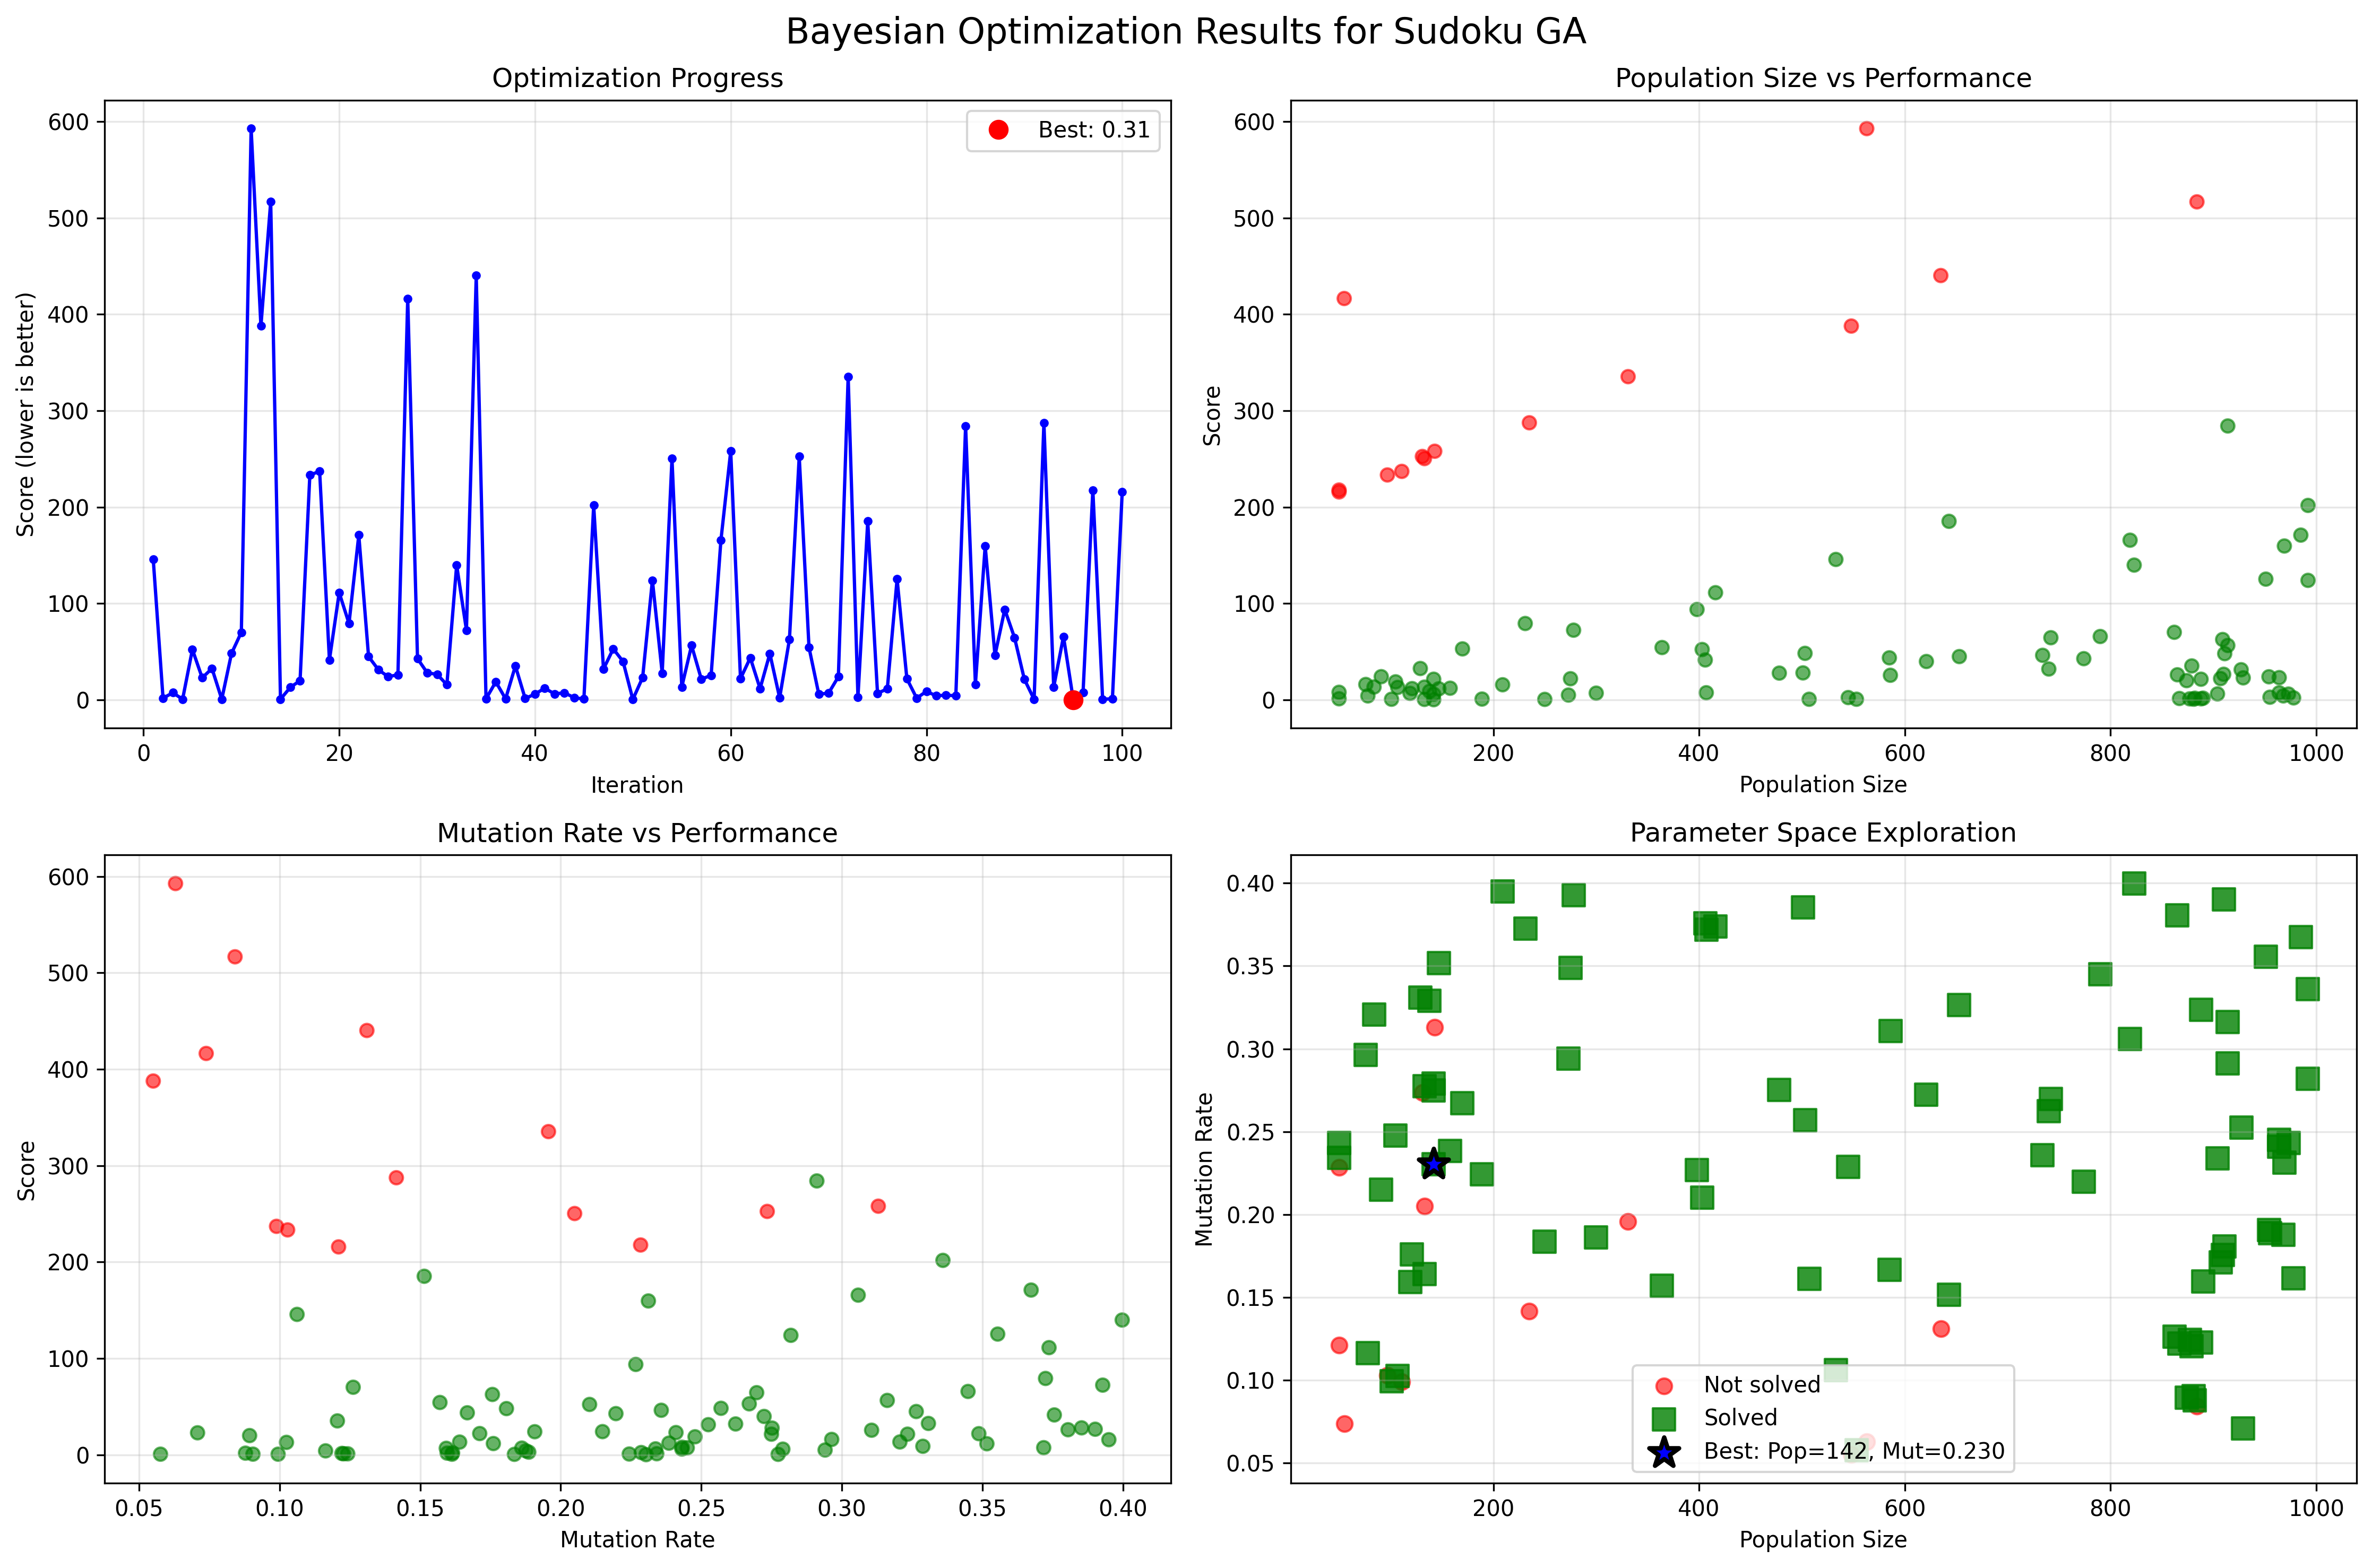
\includegraphics[width=0.8\textwidth]{resources/bayesian_optimization_results.png}
\caption{Bayesian optimization results.}
\label{fig:bayesian_optimization_results}
\end{figure}

\subsection{Test the performance of the GA with varied difficulty}

We test easy, medium and hard difficulty in same setting, and it's costly to test 1000 times for each difficulty. Thus we only test easy difficulty for 1000 times, medium one for around 400 times, and hard one for 100 times.

\subsubsection{Easy difficulty}

The charts below shows the performance of the GA with easy difficulty. There are more than 500 times find solution in less than 0.5 seconds. only around $1/20$ solutions were reached very slow which is more than 20s.
Additionly, the average execution time is 5s-ish, which is a good performance. Moreover, the execution time and generation have linear relationship. It means that if algorithm need more generations to get the solution, the more execution time it will cost.

\begin{figure}[h]
\centering
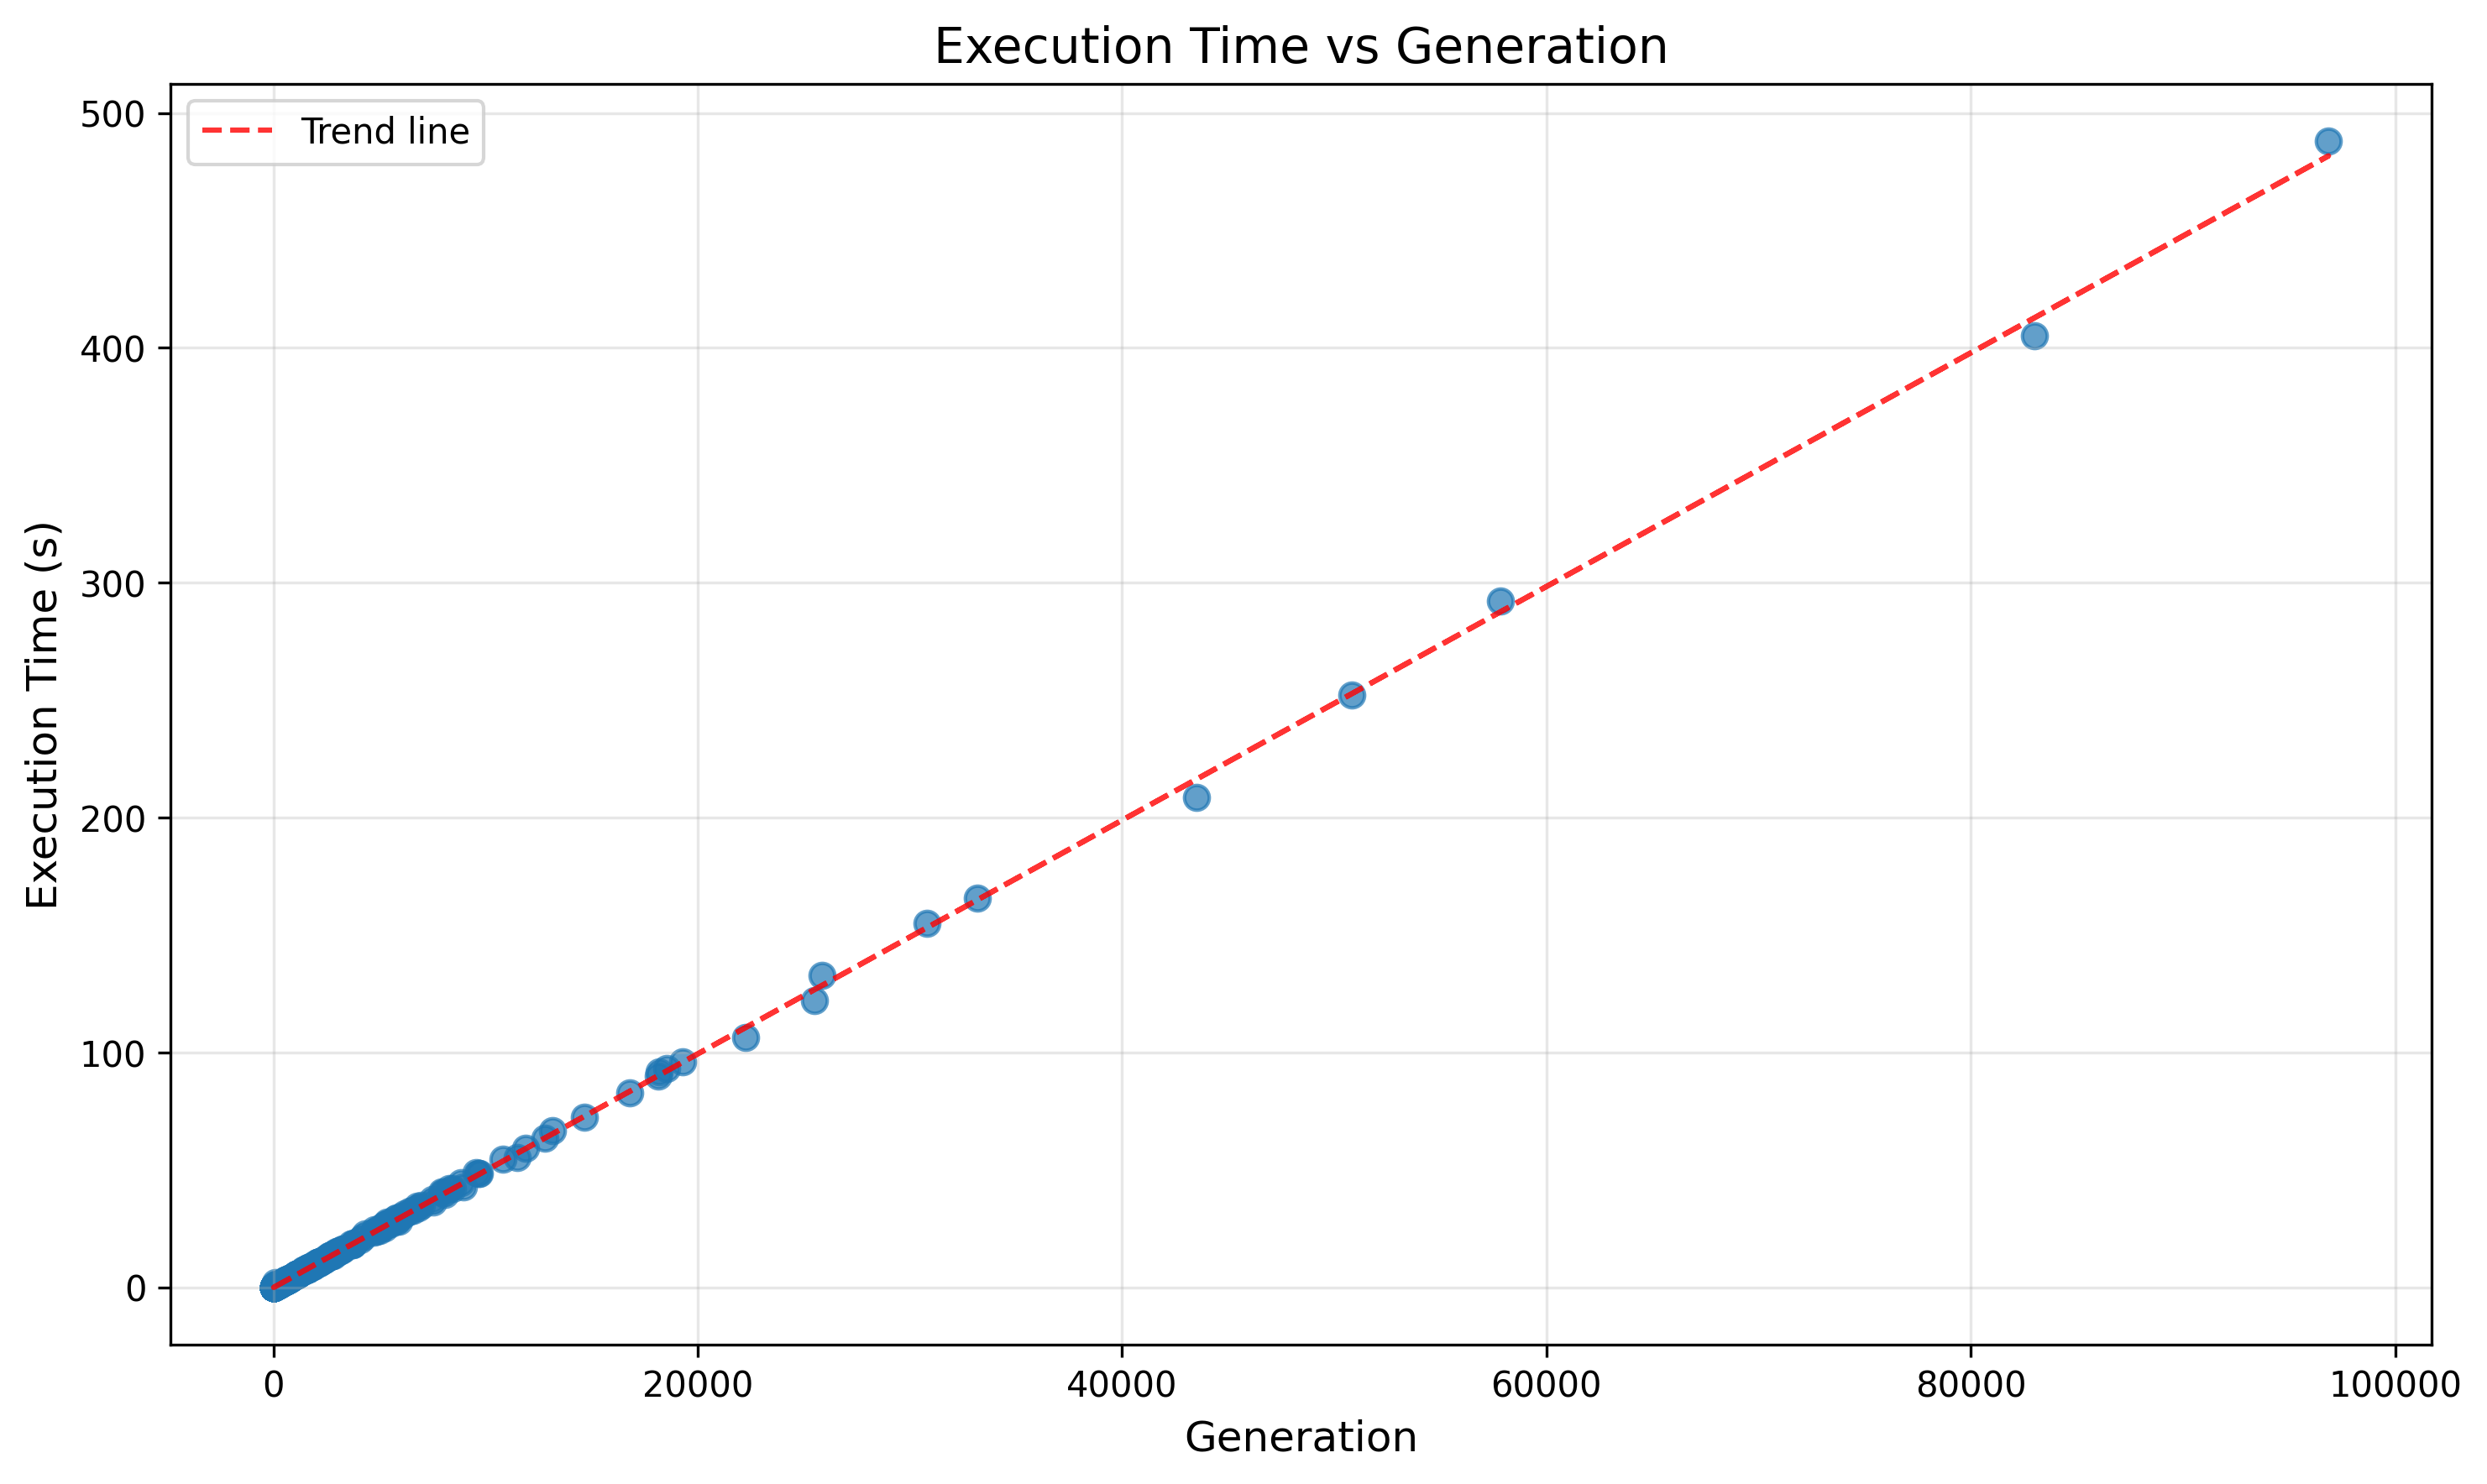
\includegraphics[width=0.8\textwidth]{resources/generation_vs_execution_time_easy.png}
\caption{Generation vs execution time for easy difficulty puzzles.}
\label{fig:generation_vs_execution_time_easy}
\end{figure}

\begin{figure}[h]
\centering
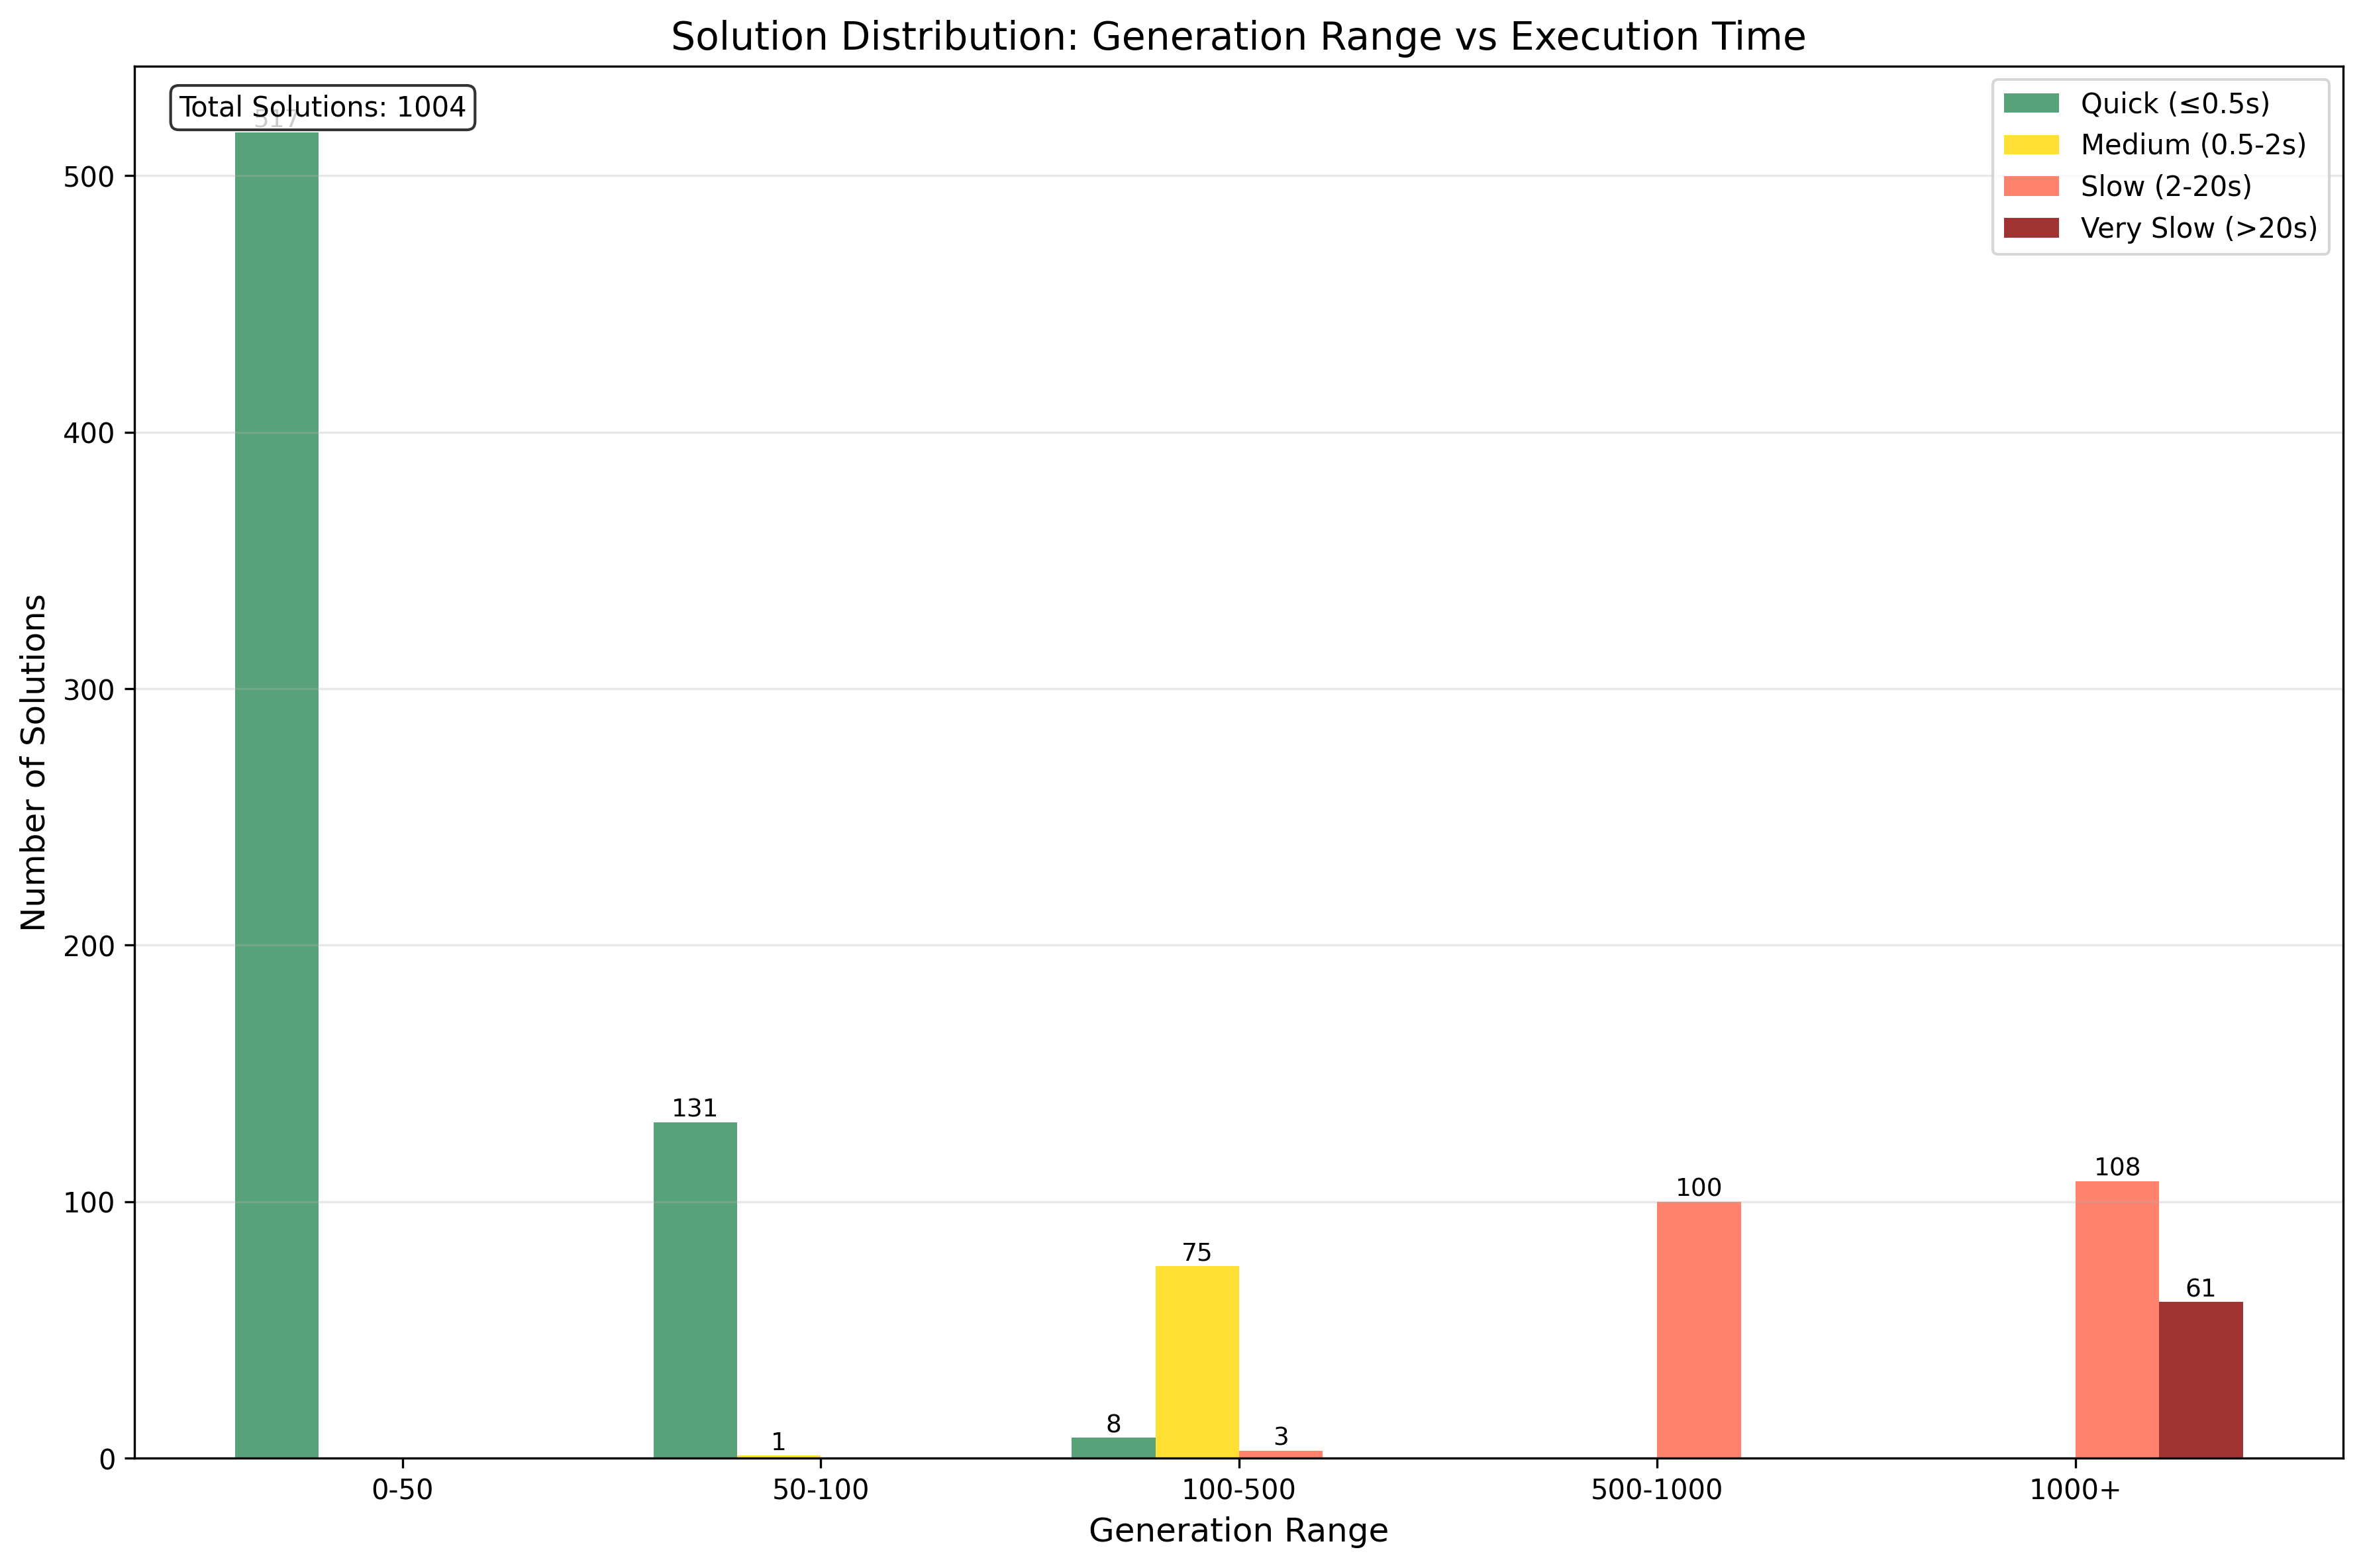
\includegraphics[width=0.8\textwidth]{resources/generation_execution_time_bars_easy.png}
\caption{Generation and execution time distribution for easy difficulty puzzles.}
\label{fig:generation_execution_time_bars_easy}
\end{figure}

\subsubsection{Medium difficulty}

The charts below shows the performance of the GA with medium difficulty, the time cost of founding solution at quick and medium time only play a small role in total cases.
However, the proportion of the getting solution in very slow is $60\%$, which is much higher comparing with easy difficulty.
Meanwhile, the execution time and generation still remain a linear relationship.

\begin{figure}[h]
\centering
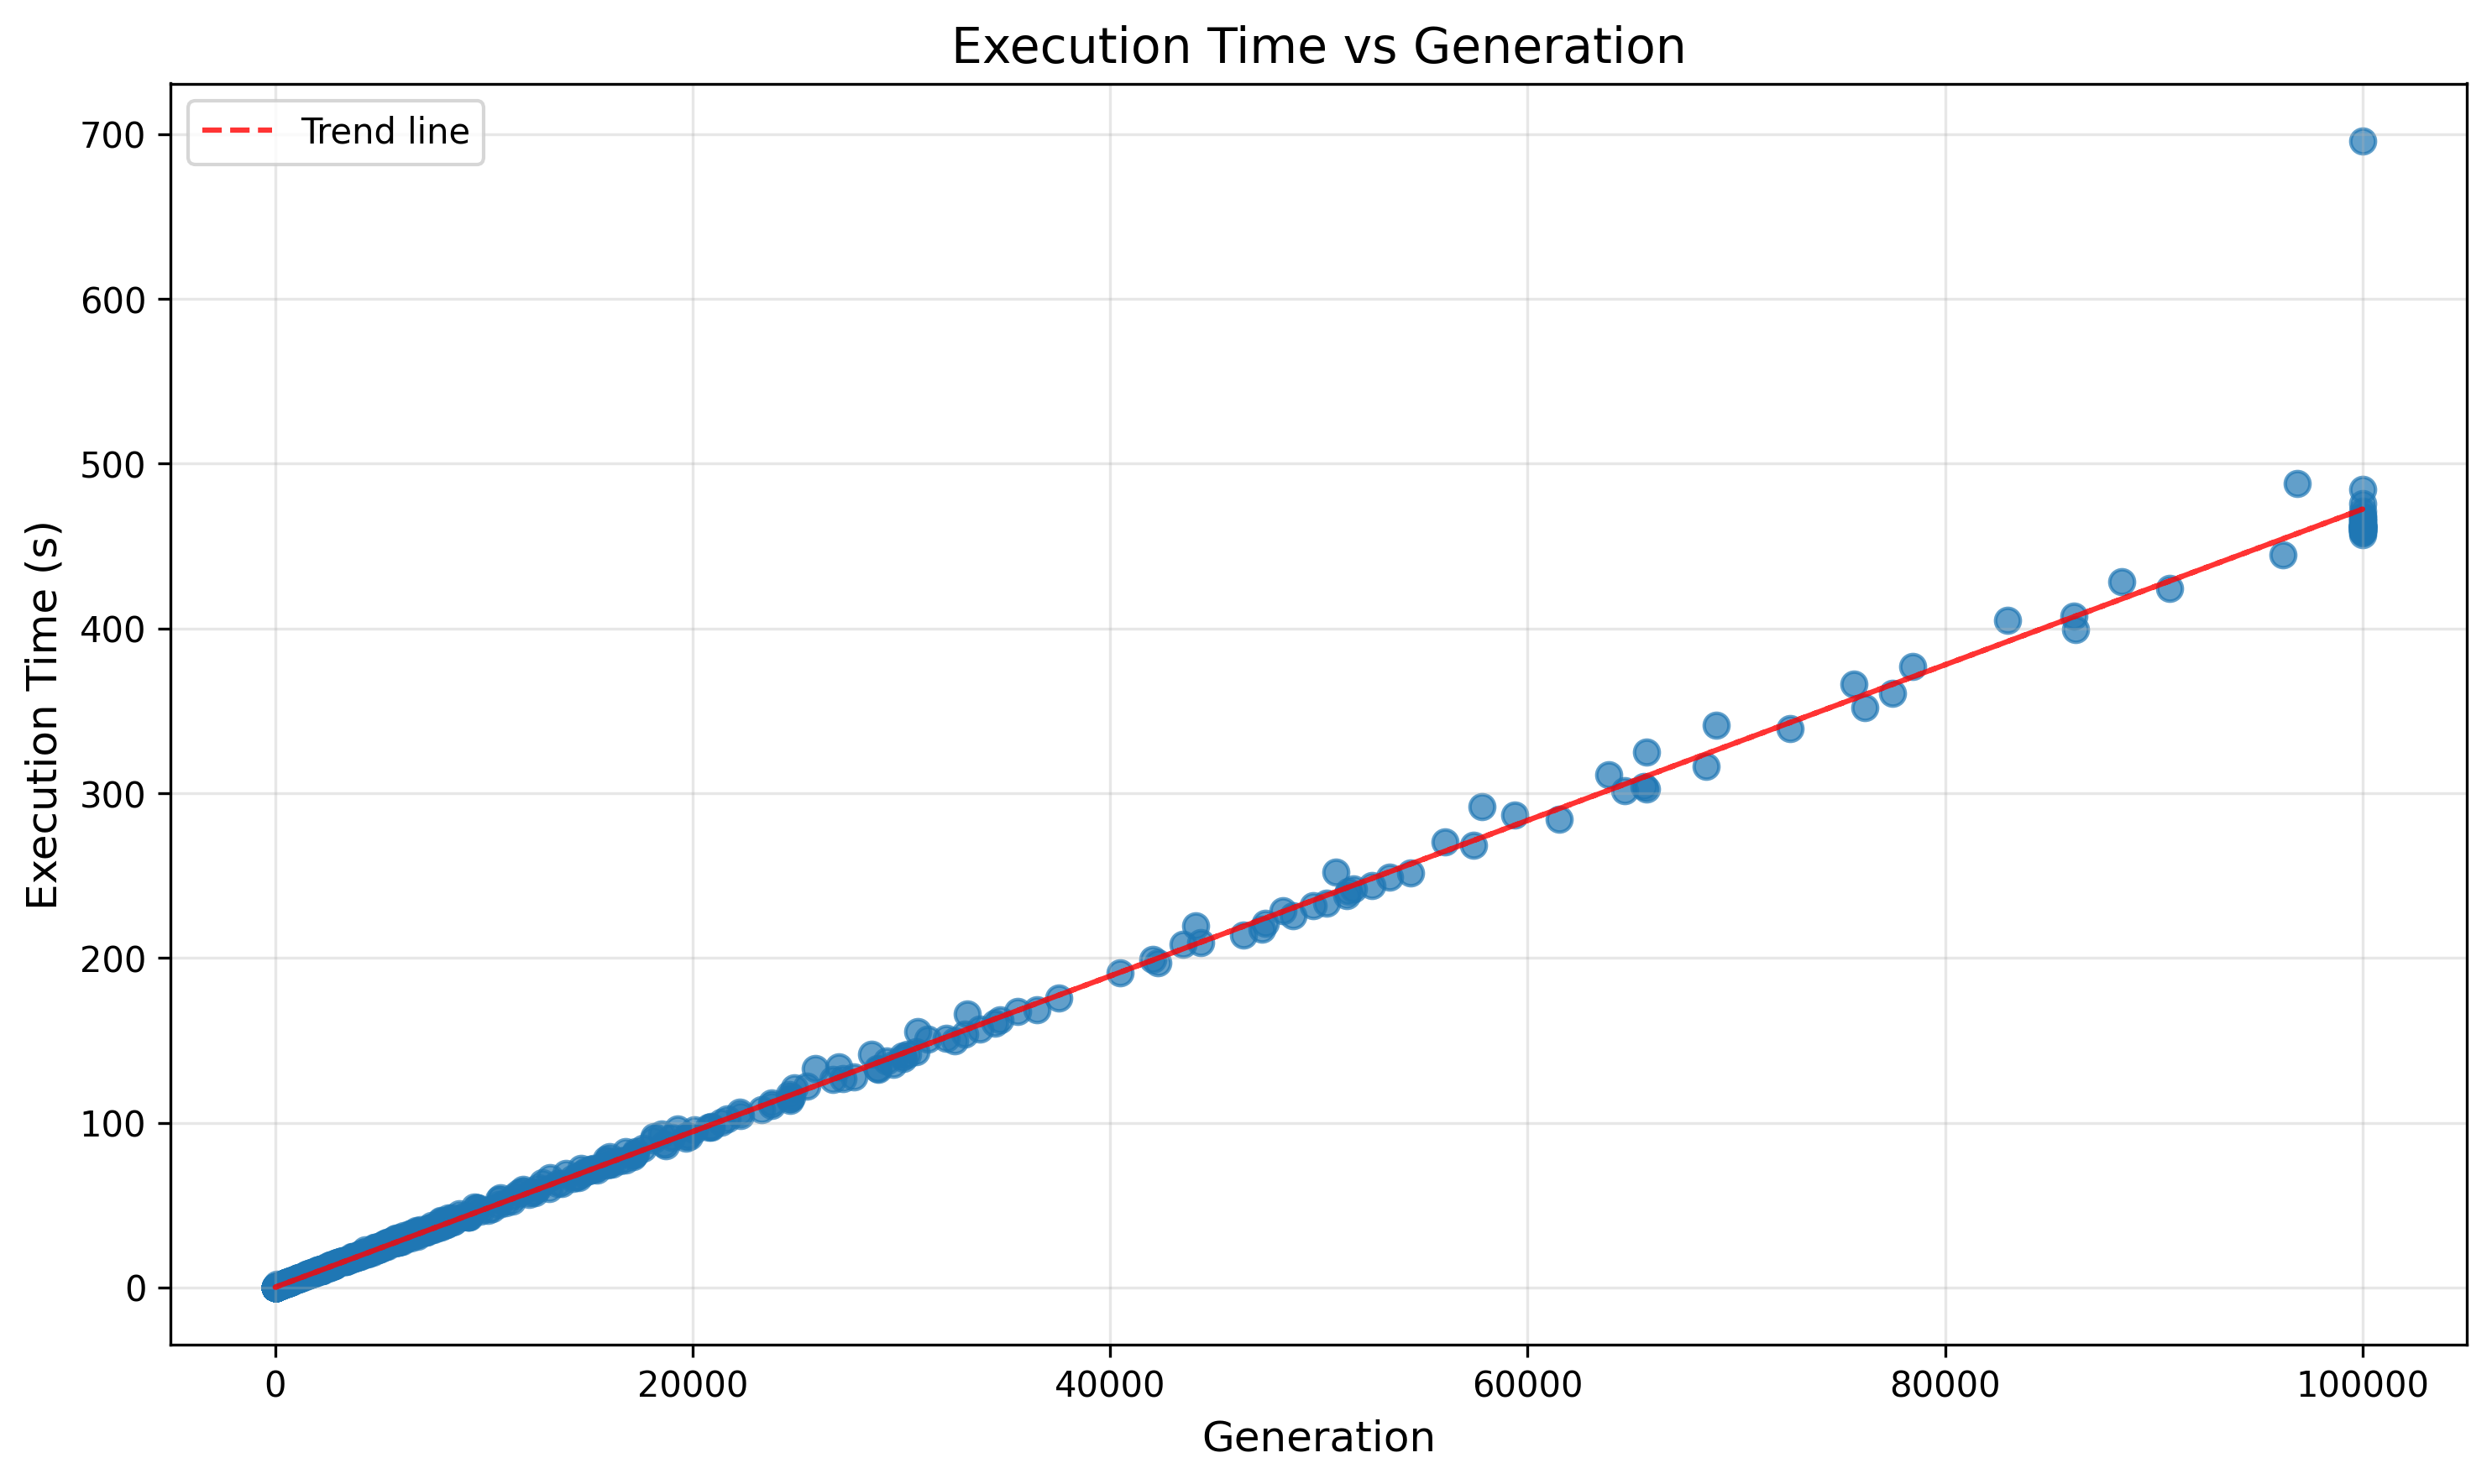
\includegraphics[width=0.8\textwidth]{resources/generation_vs_execution_time_medium.png}
\caption{Generation vs execution time for medium difficulty puzzles.}
\label{fig:generation_vs_execution_time_medium}
\end{figure}

\begin{figure}[h]
\centering
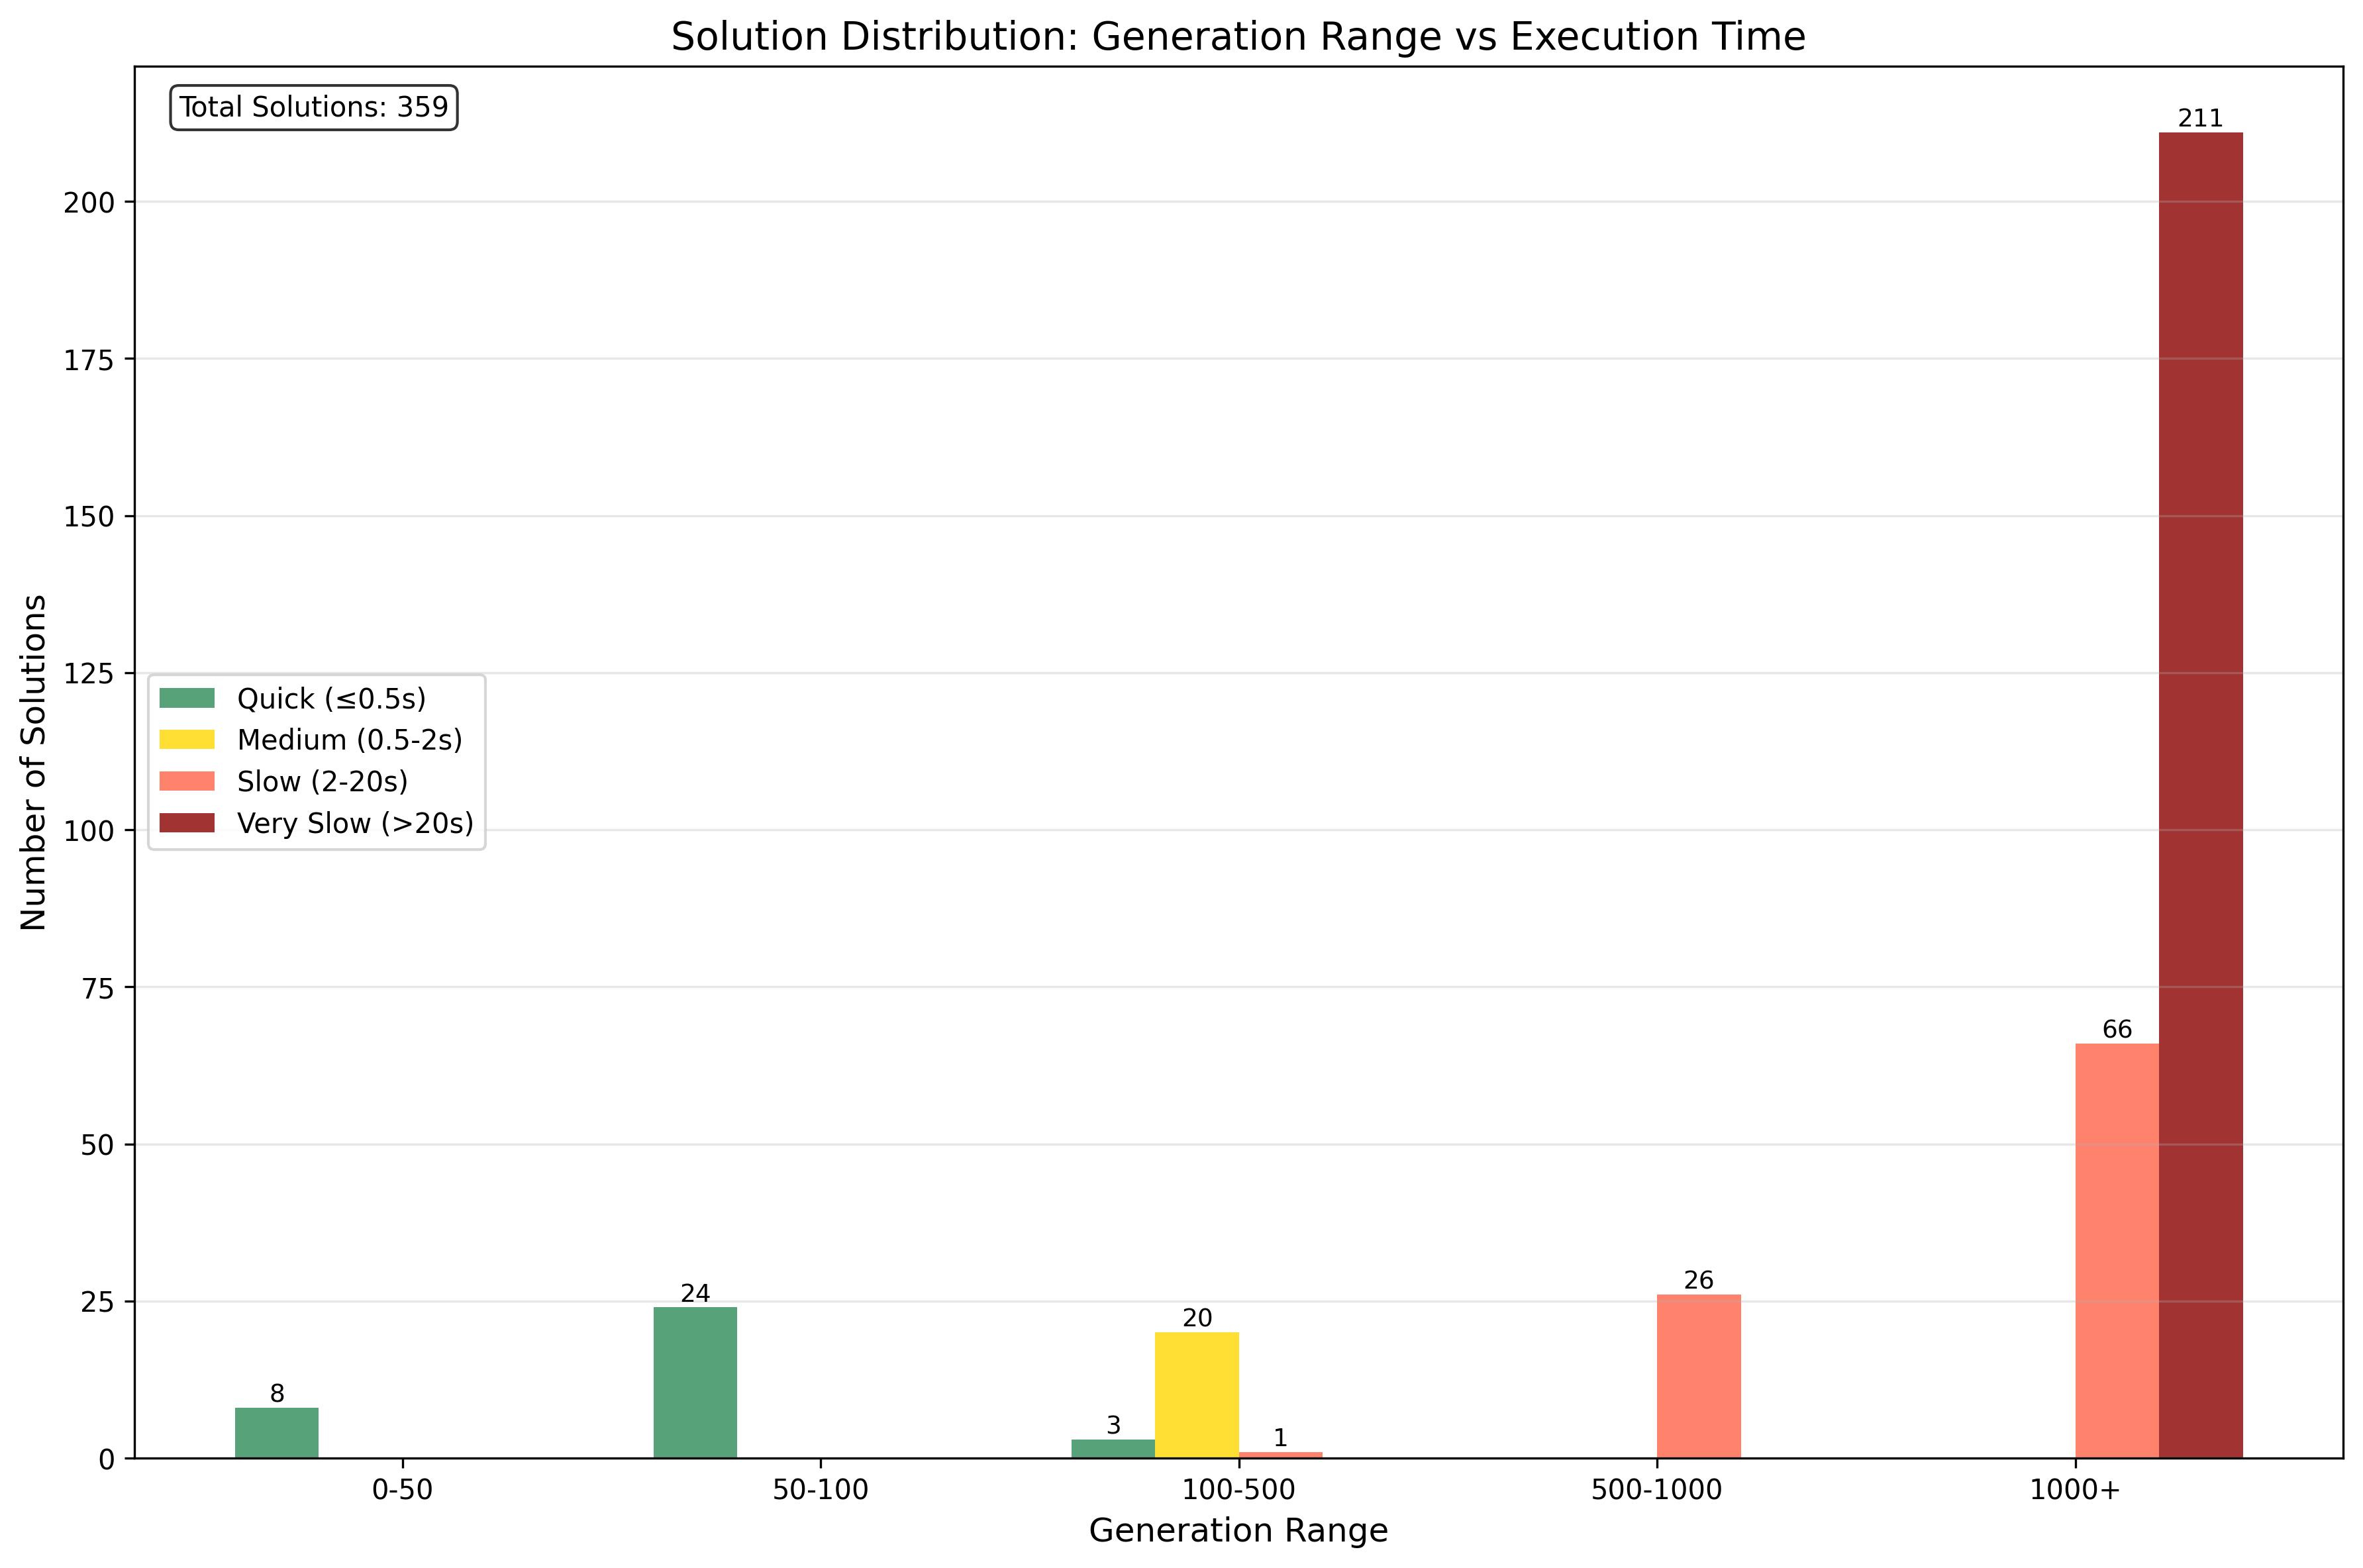
\includegraphics[width=0.8\textwidth]{resources/generation_execution_time_bars_medium.png}
\caption{Generation and execution time distribution for medium difficulty puzzles.}
\label{fig:generation_execution_time_bars_medium}
\end{figure}

\subsubsection{Hard difficulty}

The charts below shows the performance of the GA with hard difficulty, the proportion of the getting solution in very slow is $97\%$, which is much higher comparing with easy and medium difficulty.
Meanwhile, the execution time and generation still remain a linear relationship.

\begin{figure}[h]
\centering
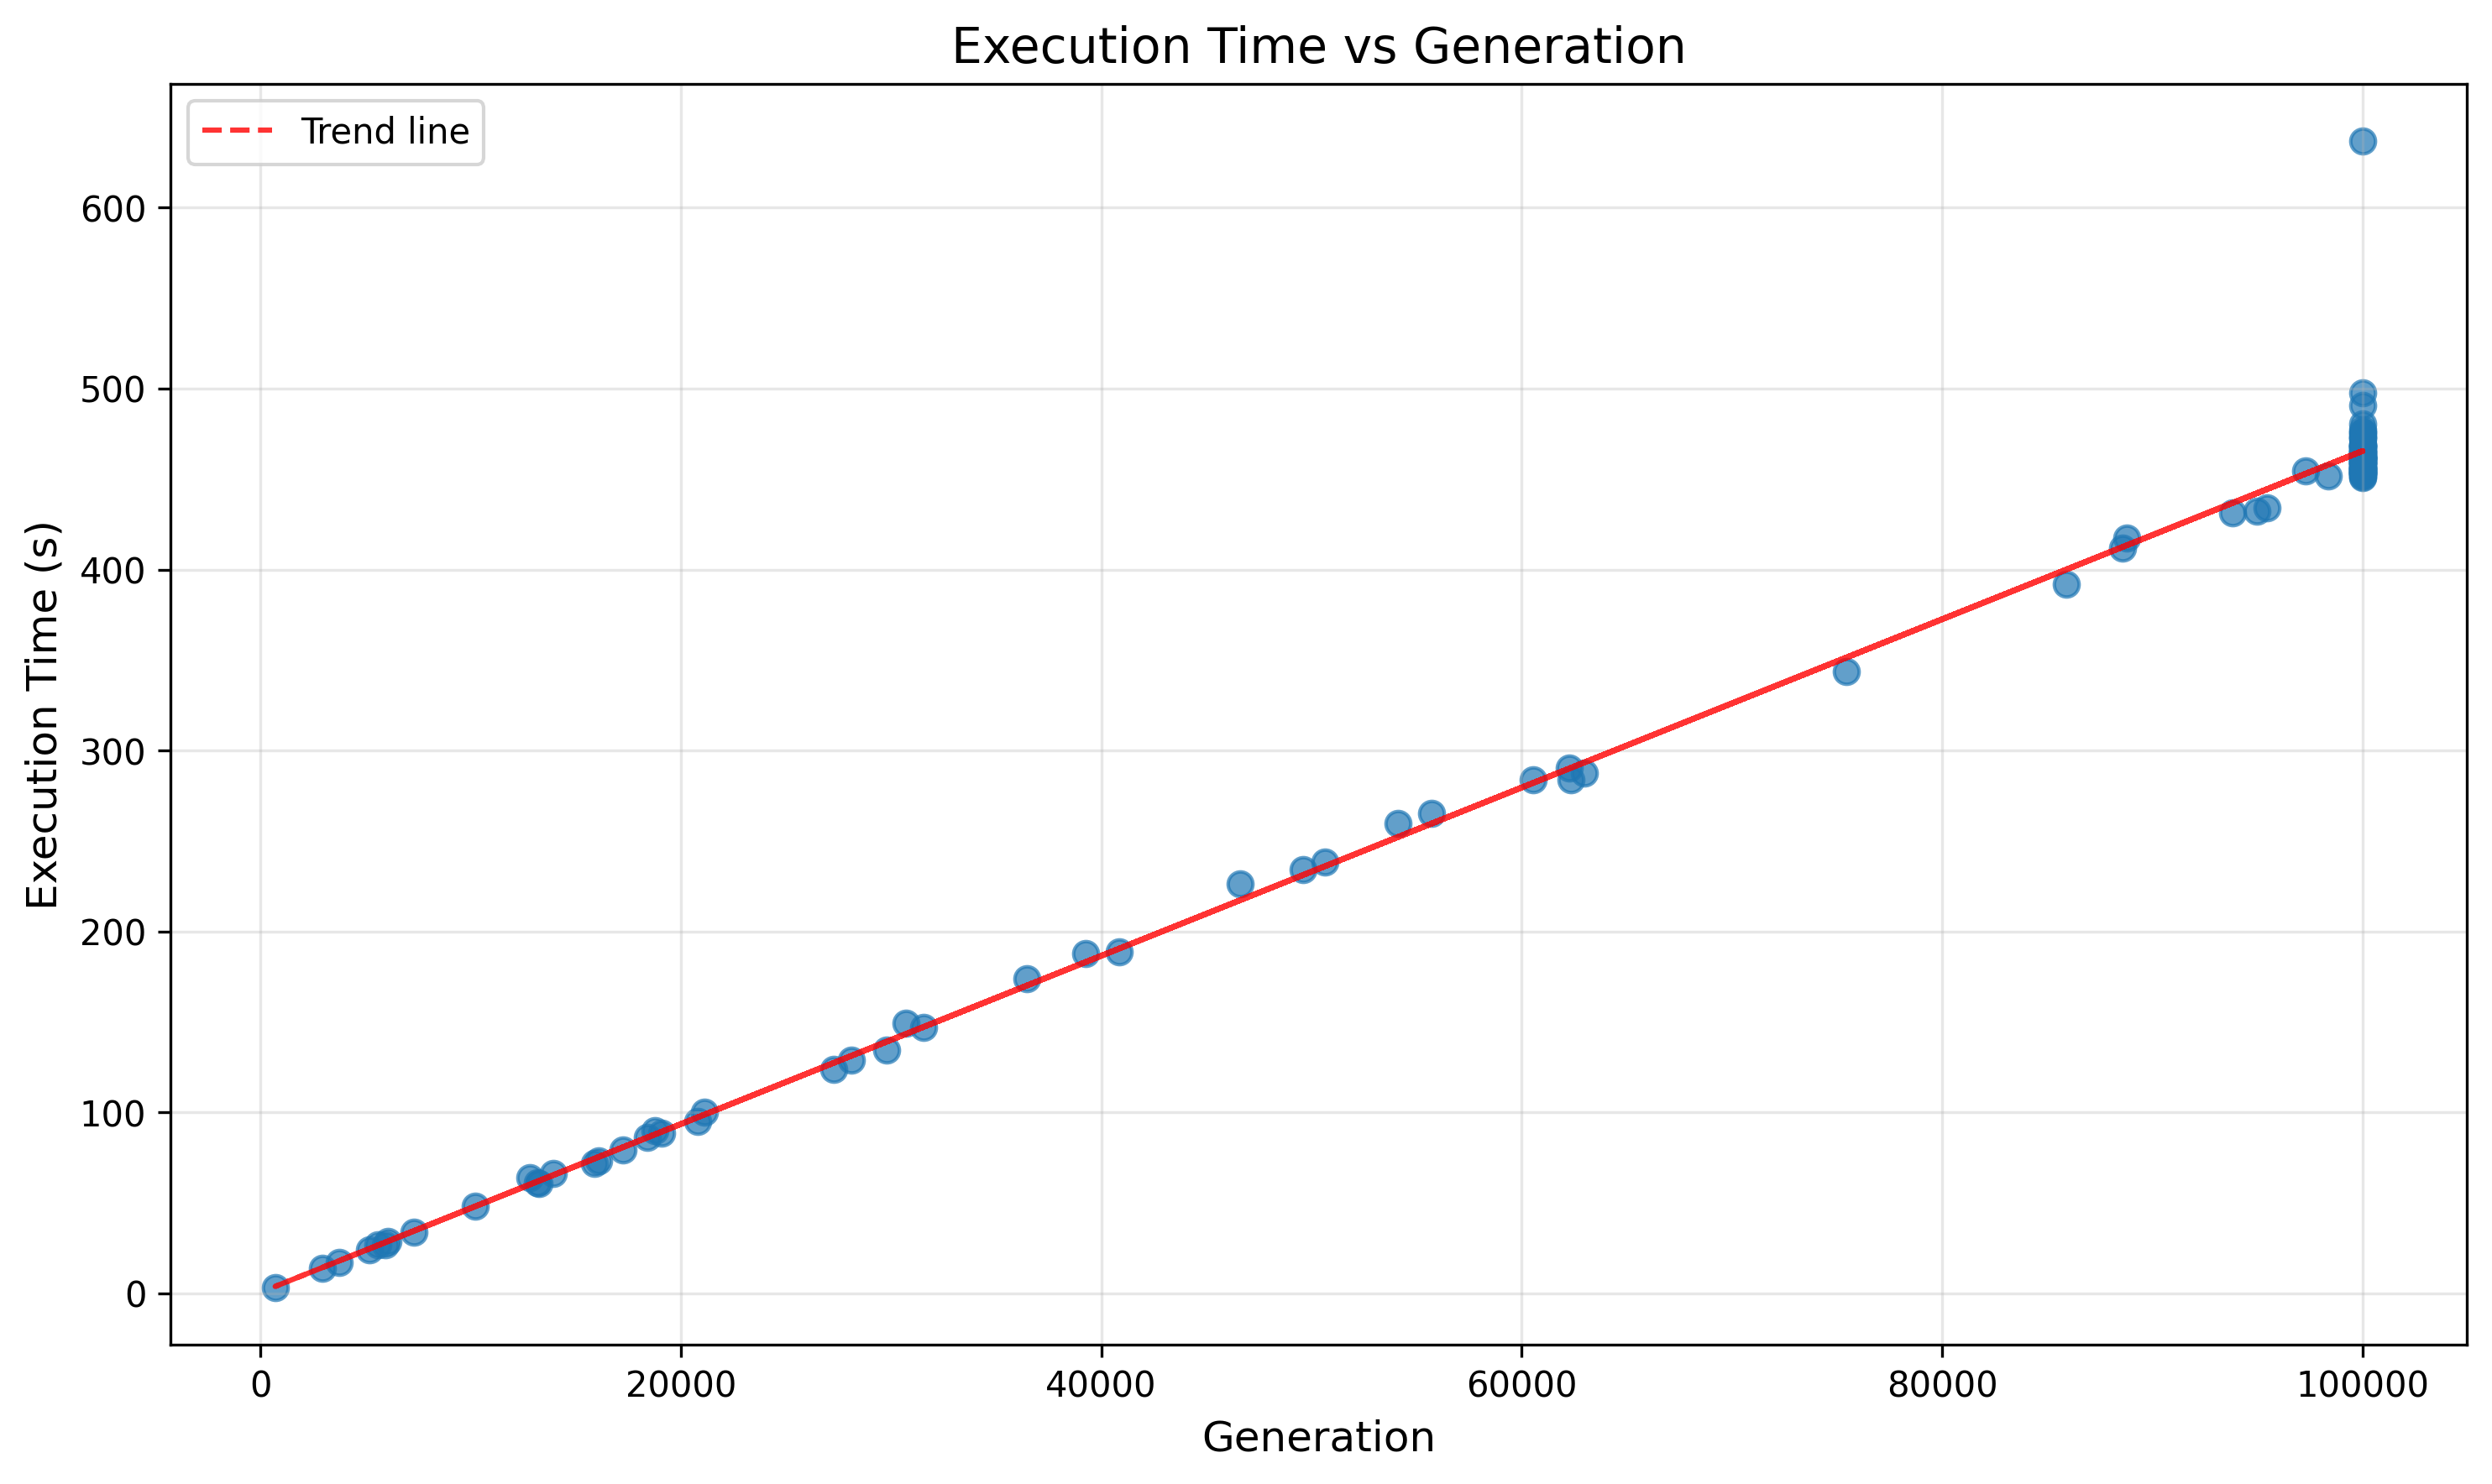
\includegraphics[width=0.8\textwidth]{resources/generation_vs_execution_time_hard.png}
\caption{Generation vs execution time for hard difficulty puzzles.}
\label{fig:generation_vs_execution_time_hard}
\end{figure}

\begin{figure}[h]
\centering
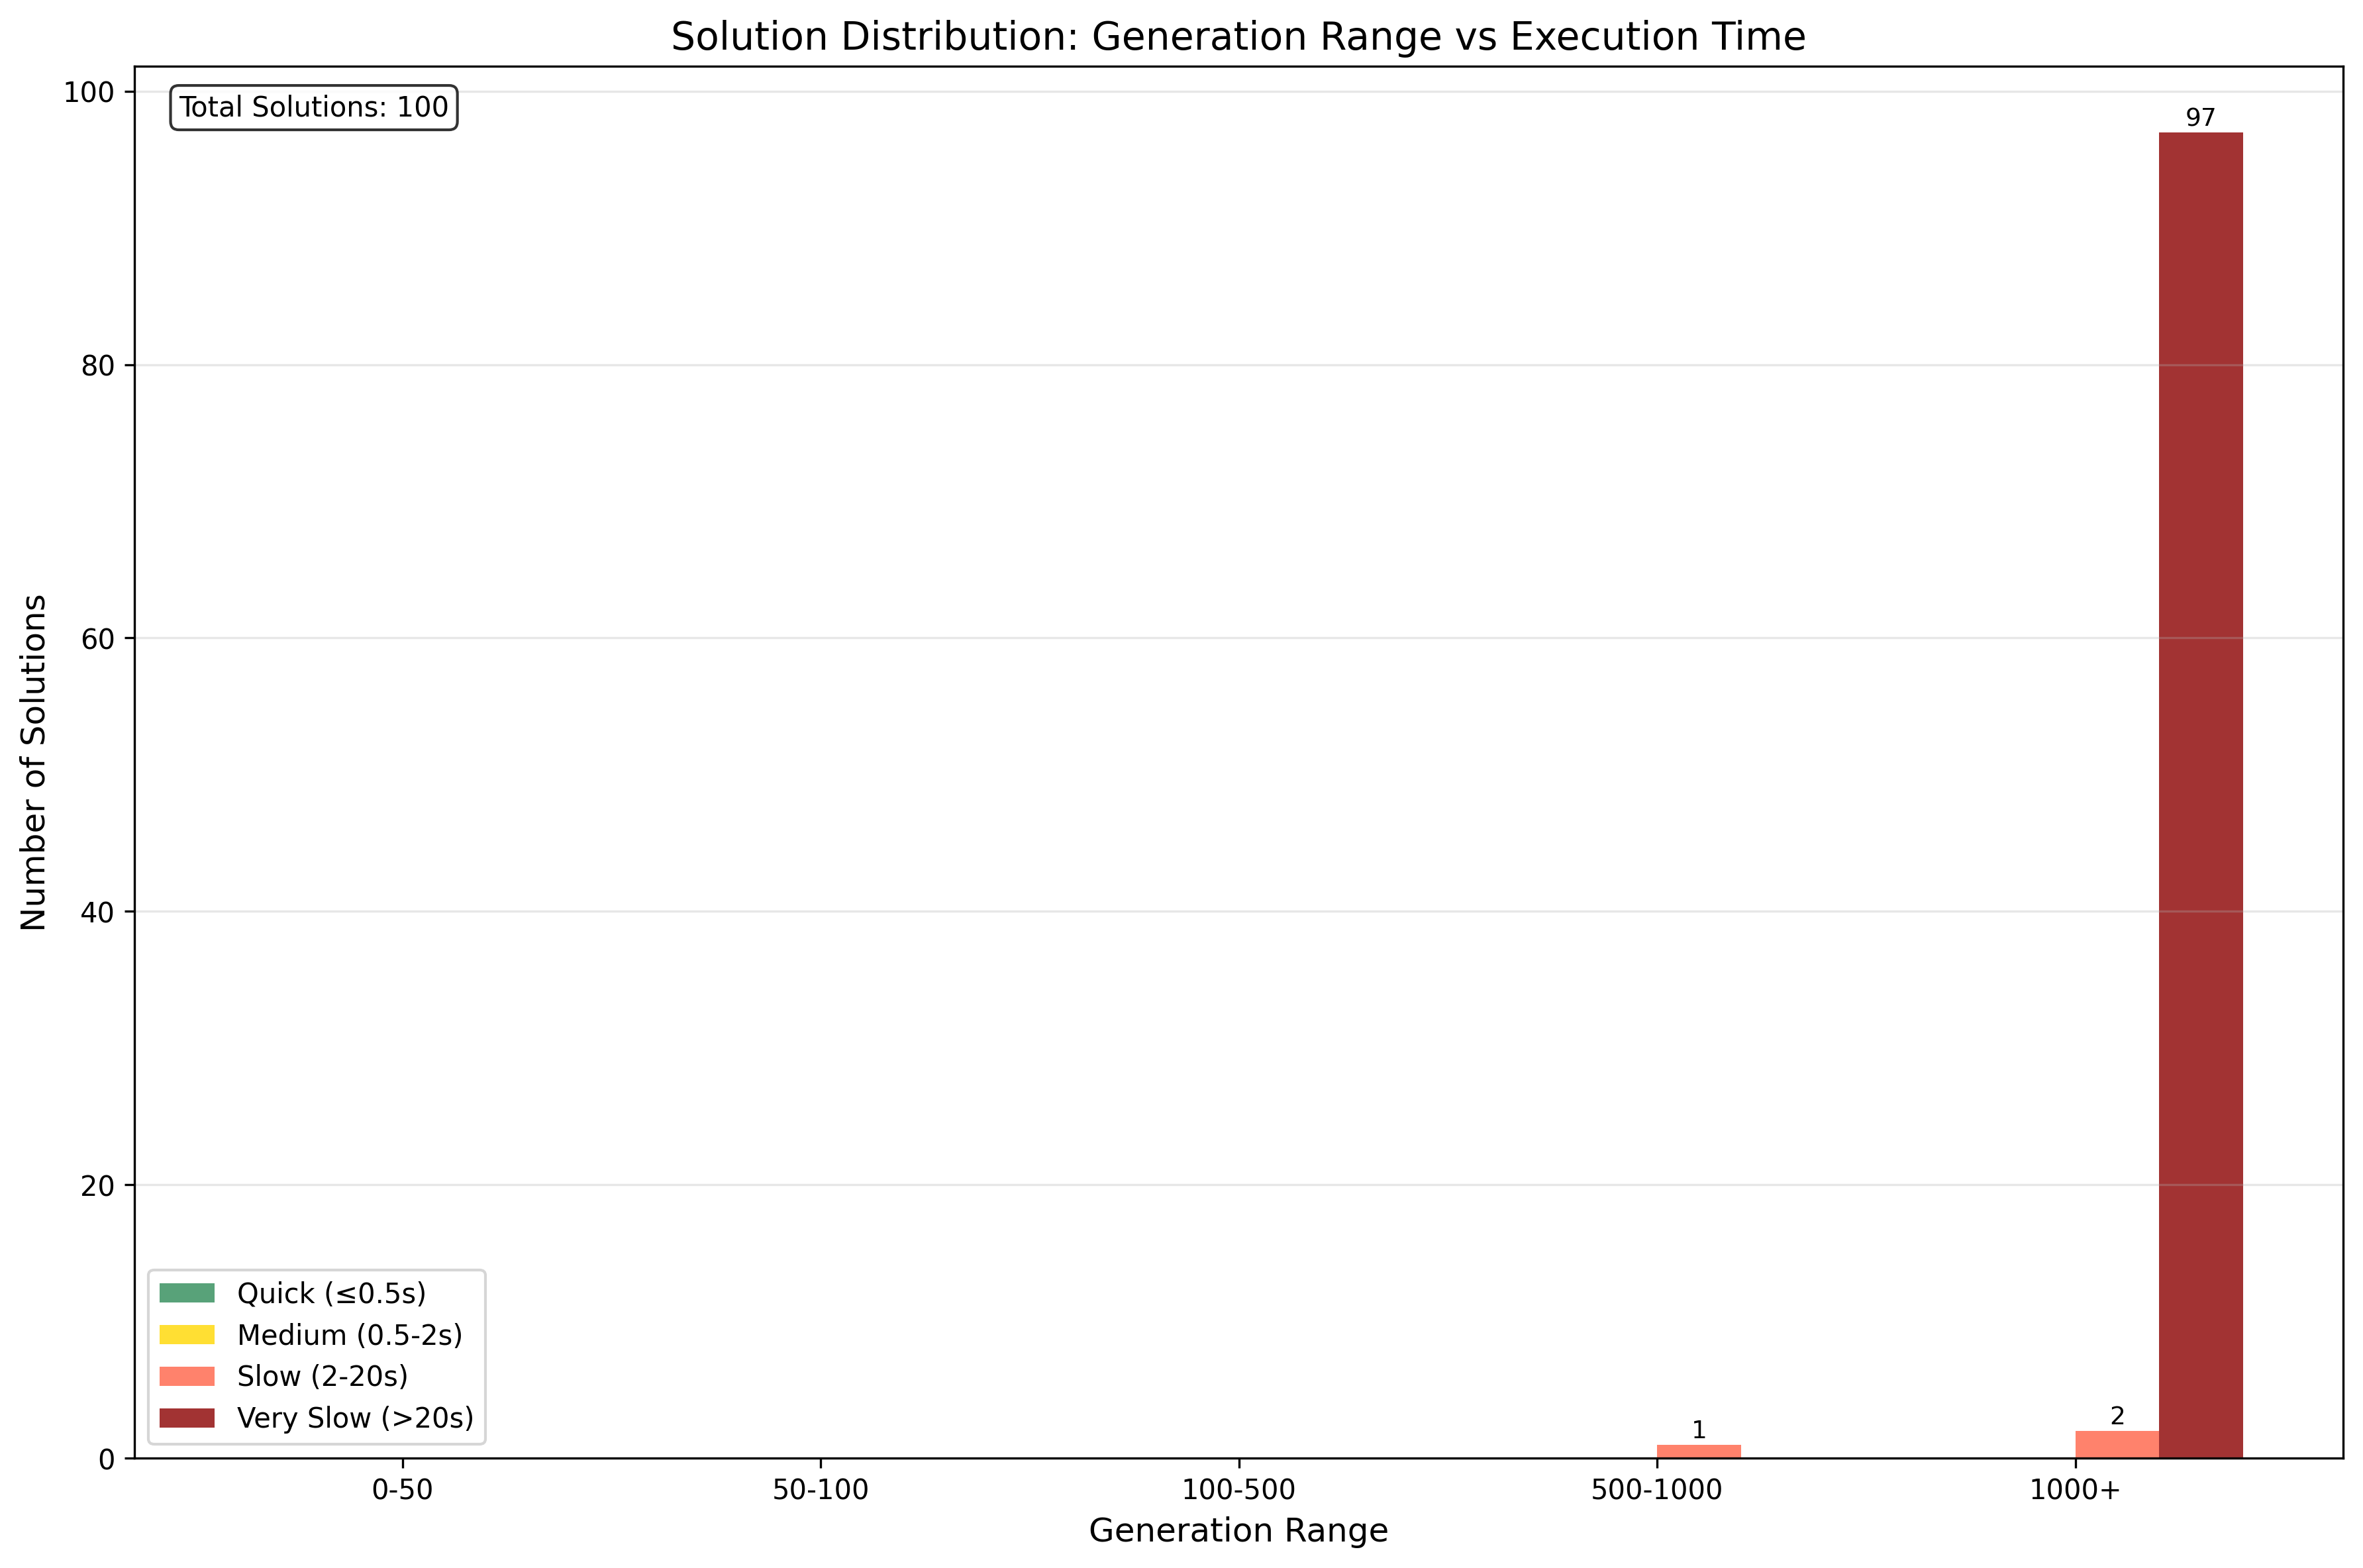
\includegraphics[width=0.8\textwidth]{resources/generation_execution_time_bars_hard.png}
\caption{Generation and execution time distribution for hard difficulty puzzles.}
\label{fig:generation_execution_time_bars_hard}
\end{figure}

\subsection{Test the performace by rule based algorithm}

We test the performace of the rule based algorithm with easy, medium and hard difficulty.

\begin{figure}[h]
\centering
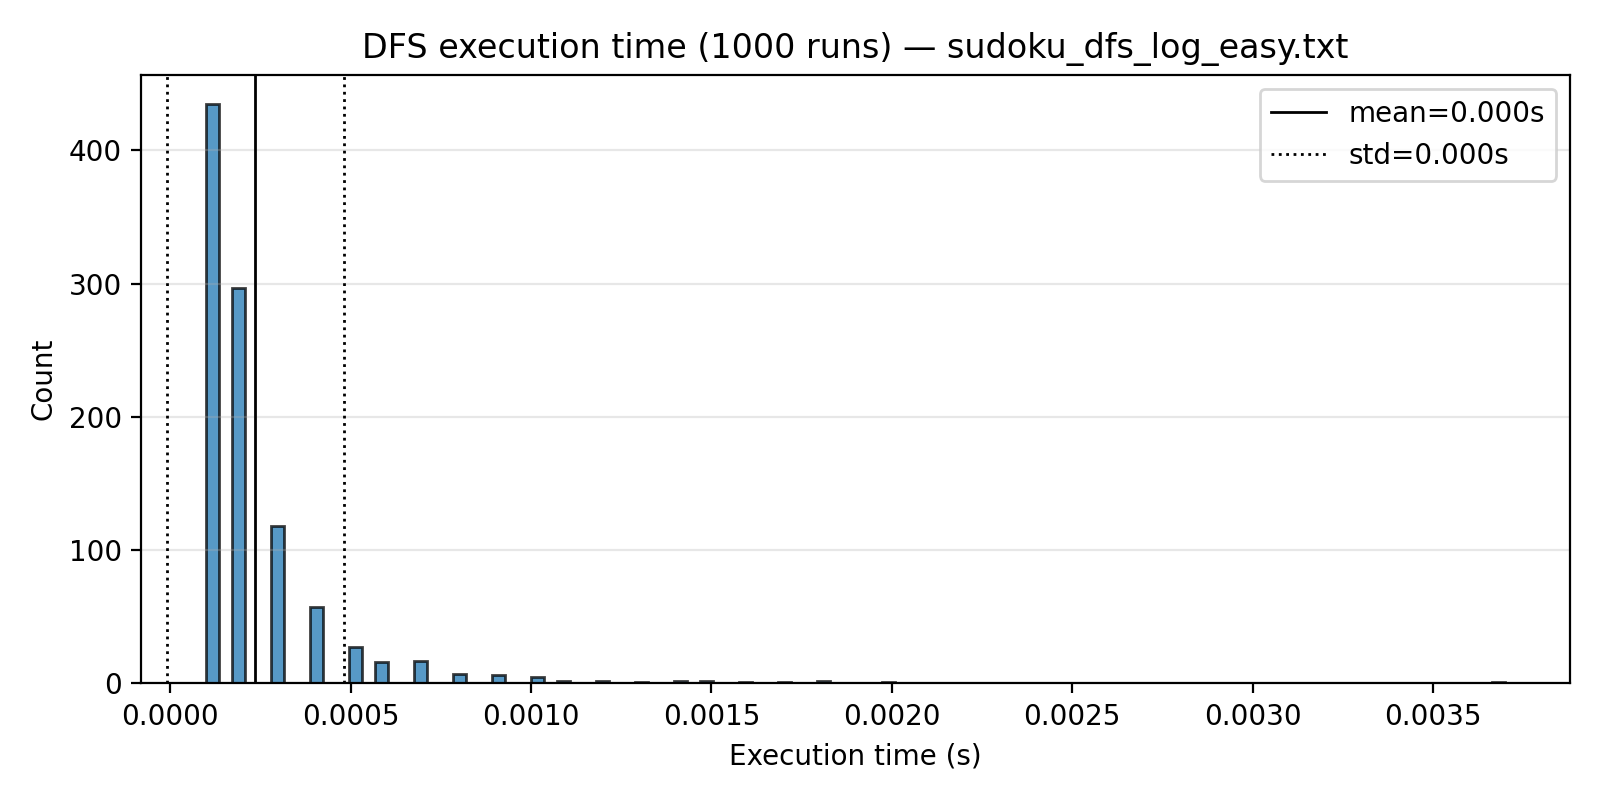
\includegraphics[width=0.8\textwidth]{resources/sudoku_dfs_log_easy_histogram.png}
\caption{Sudoku DFS log easy histogram.}
\label{fig:sudoku_dfs_log_easy_histogram}
\end{figure}

\begin{figure}[h]
\centering
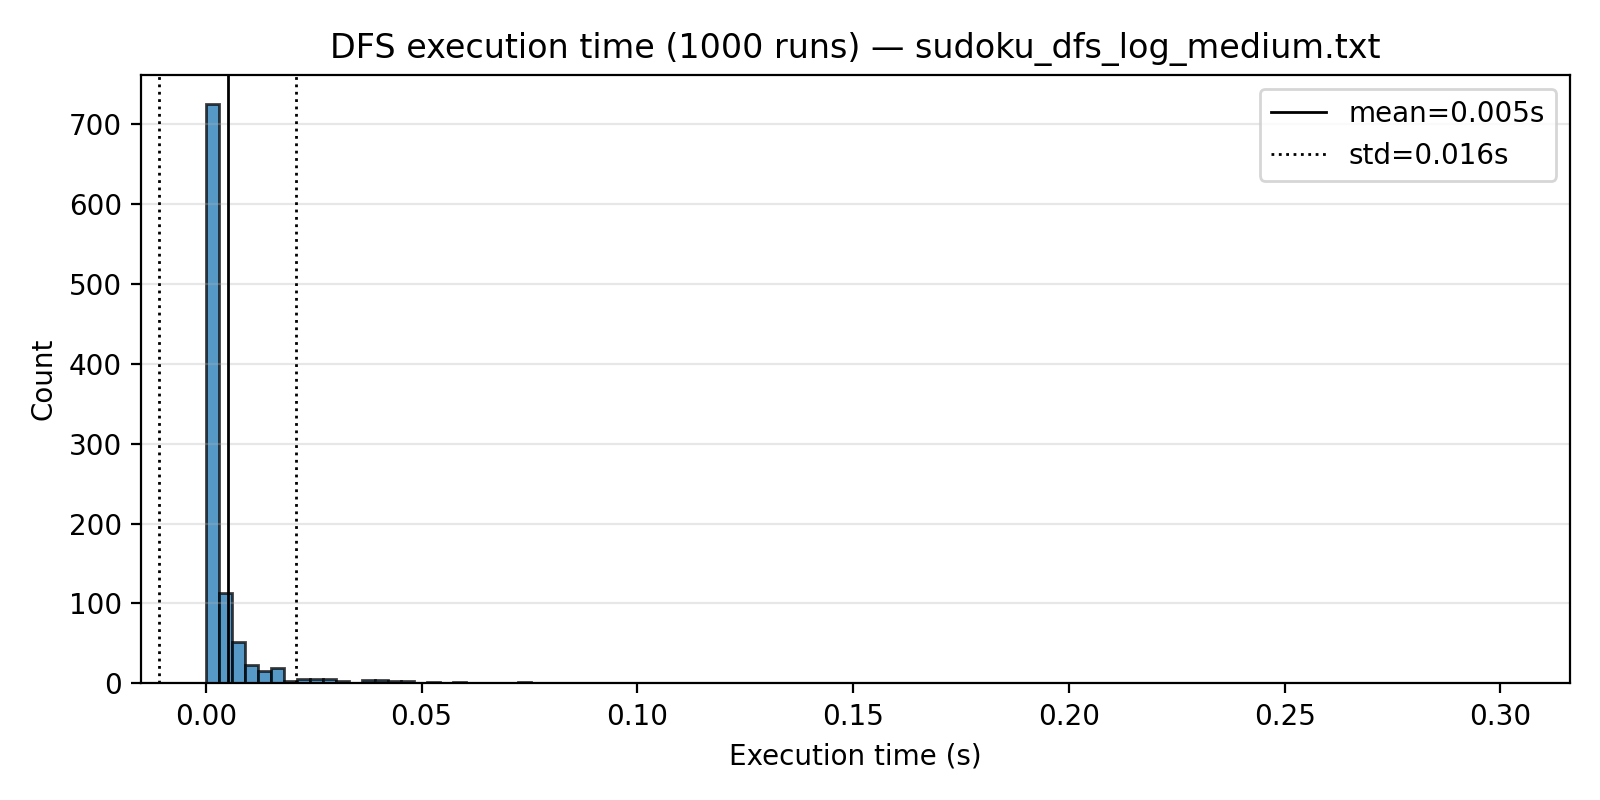
\includegraphics[width=0.8\textwidth]{resources/sudoku_dfs_log_medium_histogram.png}
\caption{Sudoku DFS log medium histogram.}
\label{fig:sudoku_dfs_log_medium_histogram}
\end{figure}

\begin{figure}[h]
\centering
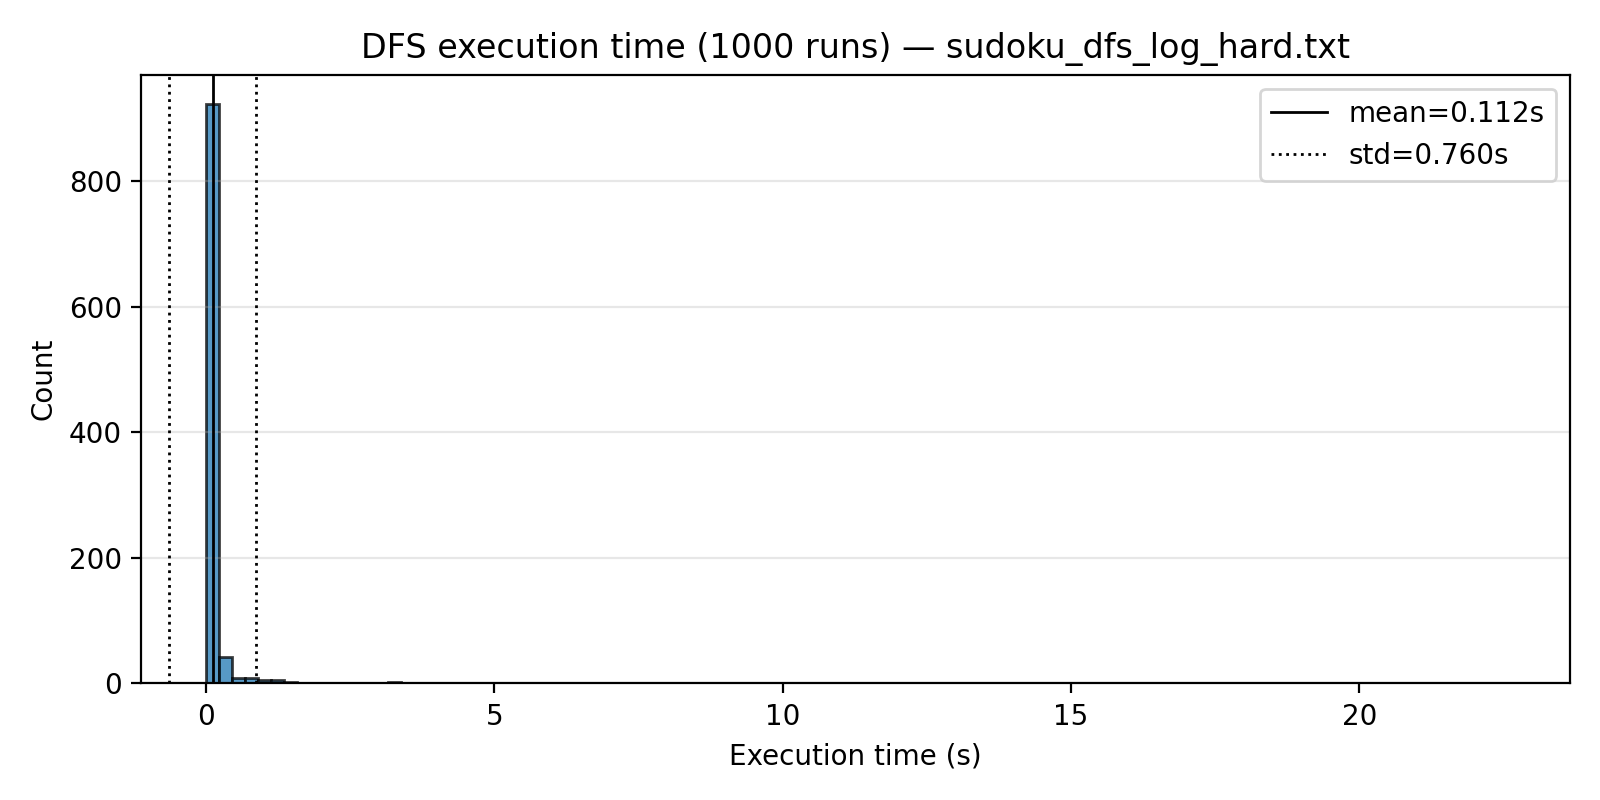
\includegraphics[width=0.8\textwidth]{resources/sudoku_dfs_log_hard_histogram.png}
\caption{Sudoku DFS log hard histogram.}
\label{fig:sudoku_dfs_log_hard_histogram}
\end{figure}

The charts illustrate that no matter how hard the puzzle is, the rule based algorithm can solve it in a short time. Moreover, the execution time is very stable, only takes 0.001s-0.002s to solve each puzzle.

\section{Conclusions}
\label{sec:conclusions}

This paper studied the efficiency of solving Sudoku puzzles with GA approaches of different complexities. The results show that the performance on 9x9 boards varies drastically. While most easy boards can be solved fast, the algorithm struggles on medium and hard boards. Only 10\% of medium boards can be solved in under 2 second. For puzzles of hard difficulties the algorithm did not achieve a single solution in under 2 seconds. Additionally, the success rate of the GA in finding a solution to the puzzle decreased with increasing complexity of the problem. While 100\% of the easy boards were solved, only 91.4\% and 45\% of boards were solved of medium and hard complexity respectively. 

The naive search algorithm DFS found solutions for every puzzle of every difficulty. Furthermore, the mean solving time of the boards of hard difficulty is 0.112 seconds, while easier puzzles were solved even faster. 

These results show that while GAs can be used to solve Sudoku puzzles, they do not outperform naive search approaches. This is the case in the Sudoku context because there is only one optimal solution (solving the board without any duplicates). GAs are not optimal. They perform well in finding solutions that are "good enough". When solving Sudokus however, only the optimal solution is relevant. The algorithm finds local maxima quickly, but then gets stuck in those in many cases. The algorithm reacts by soft resetting the population. This is done by generating a new population and combining it with some of the worst performing individuals of the stuck generation. This helps the algorithm to get out of a local maximum, but it doesn't guarantee to find the optimal solution next. This is the reason why 55\% of hard difficulty boards could not be solved in 100.000 generations.

This led to the decision of not evaluating the performance of the bigger $16 \times 16$ and $25 \times 25$ boards in this paper. It is expected that the performance of bigger grids is even worse, especially since the increase in complexity is far greater when increasing the size of the boards compared reducing given numbers in a $9 \times 9$ puzzle.

Future research may consist of combining GAs with different optimization approaches. If a significant increase in performance on 9x9 boards can be achieved, these hybrid GAs may be suitable for solving bigger $16 \times 16$ and $25 \times 25$ Sudoku puzzles.

% Example citation (replace with your actual reference key)
As shown in \cite{exampleReference}, evolutionary algorithms can solve Sudoku puzzles efficiently.

\bibliographystyle{ieeetr}
\bibliography{references}

\end{document}
